\documentclass{report}
\usepackage{geometry}
\usepackage{graphicx}
\usepackage{fancyhdr}
\usepackage{titlesec}
\usepackage{hyperref}
\usepackage{amsmath,amssymb,amsthm,textcomp}
\usepackage{enumerate}
\usepackage{multicol}
\usepackage{tikz}
\usepackage{geometry}
%\geometry{left=25mm,right=25mm,%
%bindingoffset=0mm, top=20mm,bottom=20mm}
\usepackage{float}
\newfloat{code}{htbp}{loc}
\floatname{code}{Code Listing}


\linespread{1.3}

\newcommand{\linia}{\rule{\linewidth}{0.5pt}}

% custom theorems if needed
\newtheoremstyle{mytheor}
    {1ex}{1ex}{\normalfont}{0pt}{\scshape}{.}{1ex}
    {{\thmname{#1 }}{\thmnumber{#2}}{\thmnote{ (#3)}}}

\theoremstyle{mytheor}
\newtheorem{defi}{Definition}

% my own titles
\makeatletter
\renewcommand{\maketitle}{
\begin{center}
\vspace{2ex}
{\huge \textsc{\@title}}
\vspace{1ex}
\\
\linia\\
\@author \hfill \@date
\vspace{4ex}
\end{center}
}
\makeatother
%%%

% custom footers and headers


% code listing settings
\usepackage{listings}
\lstset{
    language=Python,
    basicstyle=\ttfamily\small,
    aboveskip={1.0\baselineskip},
    belowskip={1.0\baselineskip},
    columns=fixed,
    extendedchars=true,
    breaklines=true,
    tabsize=4,
    prebreak=\raisebox{0ex}[0ex][0ex]{\ensuremath{\hookleftarrow}},
    frame=lines,
    showtabs=false,
    showspaces=false,
    showstringspaces=false,
    keywordstyle=\color[rgb]{0.627,0.126,0.941},
    commentstyle=\color[rgb]{0.133,0.545,0.133},
    stringstyle=\color[rgb]{01,0,0},
    numbers=left,
    numberstyle=\small,
    stepnumber=1,
    numbersep=10pt,
    escapeinside={\%*}{*)},
}


% Set page size, borders, and margins
\geometry{
    a4paper,
    left=1in,
    right=1in,
    top=1in,
    bottom=1in
}

% Define new page style with borders
\fancypagestyle{bordered}{%
    \fancyhf{} % Clear header and footer
    \renewcommand{\headrulewidth}{0pt} % Remove header rule
    \renewcommand{\footrulewidth}{0pt} % Remove footer rule
}

% Reduce font size by 10%
\titleformat{\chapter}[display]
  {\normalfont\bfseries}{}{0pt}{\centering\Huge}
%\titleformat*{\section}{\large\bfseries}
\titleformat*{\subsection}{\small\bfseries}
\titleformat*{\subsubsection}{\footnotesize\bfseries}
\usepackage{titlesec}
\titlespacing*{\chapter}{20pt}{-50pt}{10pt}
\titleformat{\section}{\large\bfseries}{\thesection}{1em}{}

\newcommand{\mychapter}[2]{
    
    \setcounter{chapter}{#1}
    \setcounter{section}{0}
    \chapter*{#2}
    %\addcontentsline{toc}{chapter}{#2}
}

\begin{document}
%\thispagestyle{bordered}

\begin{titlepage}
\centering

\textbf{\Large GOVERNMENT OF KERALA}\\
\vspace{0.85cm}
\textbf{\Large DEPARTMENT OF TECHNICAL EDUCATION}\\
\vspace{1.5cm}
\textbf{\Large RAJIV GANDHI INSTITUTE OF TECHNOLOGY}\\
\vspace{0.85cm}
\textbf{\Large (GOVT. ENGINEERING COLLEGE)}\\
\vspace{0.85cm}
\textbf{\Large KOTTAYAM - 686501}
\vspace{5.35cm}

\centerline{
\includegraphics[width=0.25\textwidth]{image.png}} % Reduce the image size by 40%

\vspace{6.5cm}

\textbf{\Large RECORD BOOK}

\vspace{0.9cm}
\newpage
\thispagestyle{empty}
\textbf{\Large GOVERNMENT OF KERALA}\\
\vspace{0.9cm}
\textbf{\Large DEPARTMENT OF TECHNICAL EDUCATION}\\
\vspace{0.9cm}
\textbf{\Large RAJIV GANDHI INSTITUTE OF TECHNOLOGY}\\
\vspace{0.9cm}

\textbf{\Large (GOVT. ENGINEERING COLLEGE)}\\
\vspace{0.9cm}

\textbf{\Large KOTTAYAM - 686501}

\vspace{1.35cm}
\centerline{
\includegraphics[width=0.25\textwidth]{image.png}} % Reduce the image size by 40%
\vspace{1cm}

\textbf{\Large 20MCA241 DATA SCIENCE LAB}
\vspace{0.45cm}

\begin{center}
\begin{tabular}{ll}
\vspace{0.45cm}

\textbf{\Large Name: Anjana A A} & \dotfill \\
\vspace{0.45cm}

\textbf{\Large Branch: Master of Computer Applications} & \dotfill \\
\vspace{0.45cm}

\textbf{\Large Semester: 3} & \dotfill \\
\vspace{0.45cm}

\textbf{\Large Roll No: 13} & \dotfill \\
\end{tabular}
\end{center}

\vspace{-0.2cm}

\textbf{\Large CERTIFIED BONAFIDE RECORD WORK DONE BY}

\vspace{0.6cm}

\textbf{\Large Reg No. } \dotfill

\begin{tabular}{ll}
& \\
& \\
& \\
\textbf{\Large } & \hspace{2.4cm} \textbf{\Large STAFF IN CHARGE} \\
\vspace{0.85cm}

& \\
\textbf{\Large INTERNAL EXAMINER} &  \hspace{2.5cm}\textbf{\Large EXTERNAL EXAMINER} \\
& \\
& \\
\end{tabular}
\end{titlepage}
\pagenumbering{roman}
\tableofcontents

% Add your table of contents and content 
\newpage
\pagenumbering{arabic}

\setcounter{page}{1}
\mychapter{1}{Assignment 1 \\ \vspace{-0.3cm} Review of python programming}
\addcontentsline{toc}{chapter}{Assignment 1 Review of python programming}

\section*{Problem Statement}
\large
Write Python code to explore and practice with the basic data types, containers, functions, and classes of Python. 

\begin{enumerate}
    \item Start by creating variables of various numeric data types and assigning them values.
    \item Print the data types and values of these variables.
    \item Perform mathematical operations on these variables.
    \item Update the values of these variables.
    \item Create boolean variables with True or False values.
    \item Print the data types of these boolean variables.
    \item Perform Boolean operations on these boolean variables.
    \item Create string variables with text values.
    \item Print the contents and lengths of these string variables.
    \item Concatenate strings.
    \item Format strings with variables.
    \item Use string methods to manipulate strings by capitalizing, converting to uppercase, justifying, centering, replacing substrings, and stripping whitespace.
    \item Create and use Python lists. Perform tasks like appending elements, indexing, slicing, and iterating through the list.
    
    \item Create and use Python tuples. Perform tasks like indexing, slicing, and concatenation.

    \item Create and use Python sets. Perform tasks like accessing, adding, deleting set elements.
    
    \item Create and use Python dictionaries. Perform tasks like adding, updating, and removing key-value pairs, and accessing values.
    
    \item Define simple functions with parameters and return values.
    \item Call functions with different arguments and use the returned results.
    \item Write functions that accept other functions as arguments.
    \item Define and use Python classes. Include tasks like creating a class, defining methods, and creating instances.
    \item Implement class inheritance and method overriding.
    \item Create a class with class variables and instance variables, and demonstrate their usage.
\end{enumerate}









\section{Basic data types}
\vspace{-.15cm}
\subsection{Numbers}
\vspace{-.75cm}
\begin{code}
\begin{lstlisting}
x = 43
print(x)
print("Addition",x + 1)   
print("Subtraction",x - 1)   
print(" Multiplication",x * 2)   
print("Exponentiation",x ** 2)  
print("Division",x / 2)  
\end{lstlisting}
\end{code}
\vspace{-1cm}
\begin{verbatim}
43 <class 'int'> 
Addition 44
Subtraction 42
Multiplication 86
Exponentiation 1849
Division 21.5
\end{verbatim}


\vspace{-.6cm}
\subsection{Booleans}
\vspace{-.75cm}
\begin{code}
\begin{lstlisting}
t, f = True, False
print(type(t))
print(t and f) # Logical AND;
print(t or f)  # Logical OR;
print(not t)   # Logical NOT;
print(t != f)  # Logical XOR;
\end{lstlisting}
\end{code}
\vspace{-1cm}
\begin{verbatim}
<class 'bool'>
False True False True
\end{verbatim}
\subsection{Strings}
\vspace{-.75cm}
\begin{code}
\begin{lstlisting}
    hello='Hello'
    world='World'
    print(hello, len(hello))
    hw = hello + ' ' + world 
    print(hw)
    hw12 = '{} {} {}'.format(hello, world, 12) 
    print(hw12)
\end{lstlisting}
\end{code}
\vspace{-1cm}
\begin{verbatim}
hello 5
hello world
hello world 12

\end{verbatim}
\vspace{-.75cm}
\begin{code}
\begin{lstlisting}
   s = "hello"
   print(s.capitalize())
   print(s.upper()) 
   print(s.rjust(7))    
   print(s.center(7)) 
  print(s.replace('l', '(ell)'))
  print('  world '.strip())
\end{lstlisting}
\end{code}
\vspace{-1cm}
\begin{verbatim}
Hello
HELLO
 hello
   hello
he(ell)(ell)o
world
\end{verbatim}
\vspace{-.75cm}
\section{Containers}
\vspace{-.4cm}
\subsection{Lists}
\vspace{-.45cm}
\begin{code}
\begin{lstlisting}
li = [2, 3, 4, 5]
print(li, li[2])
print(li[-1]) 
li[2] = 'hai'
print(li)
li.append('hello')
print(li)
r = li.pop()
print(r, li)
\end{lstlisting}
\end{code}
\vspace{-.75cm}
\begin{verbatim}
[2, 3, 4, 5] 4
5
[2, 3, 'hai', 5]
[2, 3, 'hai', 5, 'hello']
hello [2, 3, 'hai', 5]
\end{verbatim}
%\vspace{-.75cm}
\newpage
\subsection{Slicing}
\vspace{-.6cm}
\begin{code}
\begin{lstlisting}
n = list(range(6))
print(n)
print(n[1:3])
print(n[3:])
print(n[:3])
print(n[:])
print(n[:-1])
n[2:4] = [8, 9]
print(n)
\end{lstlisting}
\end{code}
\vspace{-.75cm} 
\begin{verbatim}
[0, 1, 2, 3, 4,5]
[1, 2]
[0, 1, 2]
[3, 4, 5]
[0, 1, 2, 3, 4, 5]
[0, 1, 2, 3, 4]
[0, 1, 8, 9, 4, 5]
\end{verbatim}
\vspace{-.6cm}
\subsection{Loops}
\vspace{-.6cm}
\begin{code}
\begin{lstlisting}
animals = ['cat', 'dog', 'elephent']
for animal in animals:
    print(animal)
\end{lstlisting}
\end{code}
\vspace{-1cm}
\begin{verbatim}
cat
dog
elephent
\end{verbatim}
\vspace{-.6cm}
\subsection{List comprehensions}
\vspace{-.8cm}
\begin{code}
\begin{lstlisting}
num = [ 1, 2, 3, 4, 5]
sq = []
for i in num:
    sq.append(i ** 2)
print(sq)
\end{lstlisting}
\end{code}
\vspace{-1cm}
\begin{verbatim}
[ 1, 4, 9, 16, 25]
\end{verbatim}
\vspace{-.6cm}
\subsection{Dictionaries}
\vspace{-.6cm}
\begin{code}[H]
\begin{lstlisting}
d = {'cat': 'cute', 'dog': 'furry'}
print(d['cat'])
print('cat' in d)
d['fish'] = 'wet'
print(d['fish']) 
\end{lstlisting}
\end{code}
\vspace{-1.7cm}
\begin{verbatim}
cute
True
wet
\end{verbatim}
\newpage
\vspace{-.75cm}
\subsection{Sets}
\vspace{-.75cm}
\begin{code}
\begin{lstlisting}
animals = {'cat', 'dog'}
print('cat' in animals)
print('fish' in animals)
animals.add('cat')
print(len(animals))       
animals.remove('cat')
print(len(animals))
\end{lstlisting}
\end{code}
\vspace{-1cm}
\begin{verbatim}
True
False
3
2
\end{verbatim}
\vspace{-.75cm}
\subsection{Tuples}
\vspace{-.75cm}
\begin{code}
\begin{lstlisting}
d = {(x, x + 1): x for x in range(10)}
t = (5, 6)
print(type(t))
print(d[t])       
print(d[(1, 2)])
\end{lstlisting}
\end{code}
\vspace{-.95cm}
\begin{verbatim}
<class 'tuple'>
5
1
\end{verbatim}
\vspace{-.95cm}
\section{Functions}
\vspace{-.95cm}
\begin{code}[h]
\begin{lstlisting}
def sign(x):
    if x > 0:
        return 'positive'
    elif x < 0:
        return 'negative'
    else:
        return 'zero'
for x in [-1, 0, 1]:
    print(sign(x))
\end{lstlisting}
\end{code}
\vspace{-1cm}
\begin{verbatim}
negative
zero
positive
\end{verbatim}
\newpage
\vspace{-.95cm}
\begin{code}[h]
\begin{lstlisting}
def hello(name, loud=False):
    if loud:
        print("HELLO, {}".format(name.upper()))
    else:
         print("Hello, {}!".format(name))
hello("Anjana")
hello("Ram", loud=True)
\end{lstlisting}
\end{code}
\vspace{-1cm}
\begin{verbatim}
Hello, Anjana!
HELLO, RAM
\end{verbatim}
\vspace{-.6cm}
\begin{code}[h]
\begin{lstlisting}
def apply_function(func, value):
    return func(value)
def square(x):
    return x * x
def cube(x):
    return x * x * x
print(apply_function(square, 3)) 
print(apply_function(cube, 3))    
\end{lstlisting}
\end{code}
\vspace{-1cm}
\begin{verbatim}
9
27
\end{verbatim}
\section{Classes}
\vspace{-.75cm}
\begin{code}[h]
\begin{lstlisting}
class Greeter:
    def __init__(self, name):
        self.name = name
    def greet(self, loud=False):
        if loud:
          print('HELLO, {}'.format(self.name.upper()))
        else:
          print('Hello, {}!'.format(self.name))
g = Greeter('Fred')
g.greet()
g.greet(loud=True)
\end{lstlisting}
\end{code}
\begin{verbatim}
Hello, Fred!
HELLO, FRED
\end{verbatim}
\newpage
\subsection{Inheritance and Method overriding}
\vspace{-.6cm}
\begin{code}[h]
\begin{lstlisting}
class Animal:
    def __init__(self, name):
        self.name = name

class Dog(Animal):
    def speak(self):
        return f"{self.name} barks."

class Cat(Animal):
    def speak(self):
        return f"{self.name} meows."

print(Dog("Buddy").speak())  
print(Cat("Whiskers").speak())


\end{lstlisting}
\end{code}
\vspace{-.4cm}
\begin{verbatim}
Buddy barks.
Whiskers meows.
\end{verbatim}
\subsection{Class variables and Instance variables}
\vspace{-.6cm}
\begin{code}
\begin{lstlisting}
class MyClass:
    class_var = "I am a class variable"
    def __init__(self, instance_var):
        self.instance_var = instance_var
obj = MyClass("I am an instance variable")
print(MyClass.class_var)  
print(obj.class_var)     
print(obj.instance_var)   
\end{lstlisting}
\end{code}
\begin{verbatim}
    I am a class variable
    I am a class variable
    I am an instance variable

\end{verbatim}



 

\mychapter{1}{Assignment 2 \\ \vspace{-0.3cm} Vectorized Computations using Numpy}
\addcontentsline{toc}{chapter}{Assignment 2 Vectorized Computations using Numpy}

\section*{Problem Statement}
\large
Implement the following computations using NumPy: 

\begin{enumerate}
    \item Create a matrix U of shape (m, n) with input values where m and n are input
positive integers.
    \item Compute X as the transpose of U.
      \item Create a matrix $Y$ of shape $(1, m)$ with random values $\in [0, 1]$.
    \item Create a matrix $W1$ of shape $(p, n)$ with random values $\in [0, 1]$ where $p$ is an input positive integer.
    \item Create a vector $B1$ of shape $(p, 1)$ with random values $\in [0, 1]$.
    \item Create a vector $W2$ of shape $(1, p)$ with all zeros.
    \item Create a scalar $B2$ with a random value $\in [0, 1]$.
    \item Perform the following computations iteratively 15 times:
   \begin{enumerate}
        \item $Z1 = W1 \cdot X + B1$ \hspace{0.2cm} (Matrix Multiplication)
        \item $A1 = f(Z1)$ \hspace{0.2cm} where $f$ is a function that returns 0 for negative values and the input value itself otherwise.
        \item $Z2 = W2 \cdot A1 + B2$
        \item $A2 = g(Z2)$ \hspace{0.2cm} where $g$ is a function defined as $g(x) = \frac{1}{1+e^{-x}}$.
        \item $L = \frac{1}{2} (A2 - Y)^2$
        \item $dA2 = A2 - Y$
        \item $dZ2 = dA2 \circ gprime(Z2)$ \hspace{0.2cm} where $gprime(x)$ is a function that returns $g(x) \cdot (1 - g(x))$ and $\circ$ indicates element-wise multiplication.
        \item $dA1 = W2^T \cdot dZ2$
        \item $dZ1 = dA1 \circ fprime(Z1)$ \hspace{0.2cm} where $fprime$ is a function that returns 1 for positive values and 0 otherwise and $\circ$ indicates element-wise multiplication.
        \item $dW1 = \frac{1}{m} \cdot dZ1 \cdot X^T$
        \item $dB1 = \frac{1}{m} \sum dZ1$ \hspace{0.2cm} (sum along the columns)
        \item $dW2 = \frac{1}{m} \cdot dZ2 \cdot A1^T$
        \item $dB2 = \frac{1}{m} \sum dZ2$ \hspace{0.2cm} (sum along the columns)
        \item Update and print $W1$, $B1$, $W2$, and $B2$ for $\alpha = 0.01$:
        \begin{enumerate}
            \item $W1 = W1 - \alpha \cdot dW1$
            \item $B1 = B1 - \alpha \cdot dB1$
            \item $W2 = W2 - \alpha \cdot dW2$
            \item $B2 = B2 - \alpha \cdot dB2$
        \end{enumerate}
    \end{enumerate}
\end{enumerate}









\section{Matrix}
\vspace{-.15cm}
\subsection{Create Matrix}
\vspace{-.75cm}
\begin{code}
\begin{lstlisting}
import numpy as np
m=int(input("Enter row size:"))
n=int(input("Enter column size:"))
print("Enter values in single line(space seperated formst):")
entries=list(map(int,input().split()))
U=np.array(entries).reshape(m,n)
print(U)
\end{lstlisting}
\end{code}
\vspace{-1cm}
\begin{verbatim}
Enter row size: 3
Enter column size: 3
Enter values in single line(space seperated formst):
 12 3 -8 9 34 5 6 4 54
[[12  3 -8]
 [ 9 34  5]
 [ 6  4 54]]
\end{verbatim}
\vspace{-.6cm}
\subsection{Matrix Transpose}
\vspace{-.75cm}
\begin{code}
\begin{lstlisting}
X=U.T
print("Transpose of matrix U:")
print(X) 
\end{lstlisting}
\end{code}
\vspace{-1cm}
\begin{verbatim}
Transpose of matrix U:
[[12  9  6]
 [ 3 34  4]
 [-8  5 54]]
\end{verbatim}
\vspace{-.75cm}
\newpage
\subsection{Matrix with random values}
\vspace{-.75cm}
\begin{code}
\begin{lstlisting}
m=3
Y=np.random.rand(1,m)
print(Y) 

p=int(input("Enter  positive value,p :"))
n=3
W1=np.random.rand(p,n)
print("Matrix W1\n",W1)

p=int(input("Enter a value for p :"))
B1=np.random.rand(p,1)
print("Vector B1:")
print(B1)
\end{lstlisting}
\end{code}
\vspace{-1cm}
\begin{verbatim}
[[0.1017947  0.10587389 0.76135783]]
Enter  positive value,p : 3
Matrix W1
 [[0.12742882 0.59023487 0.70840949]
 [0.12882403 0.02896318 0.7421581 ]
 [0.87475144 0.40225054 0.97983924]]
 Enter a value for p : 3
Vector B1:
[[0.89954103]
 [0.9744558 ]
 [0.59537661]]
\end{verbatim}
\vspace{-.75cm}
\subsection{Matrix with zeros}
\vspace{-.6cm}
\begin{code}
\begin{lstlisting}
p=int(input("Enter value for p :"))
W2=np.zeros((1,p))
print(W2)

\end{lstlisting}
\end{code}
\vspace{-.75cm}
\begin{verbatim}
Enter value for p : 3
[[0. 0. 0.]]

\end{verbatim}
\vspace{-.6cm}
\subsection{Scalar matrix}
\vspace{-.6cm}
\begin{code}
\begin{lstlisting}
B2=np.random.rand()
print("Scalar B2:")
print(B2)
\end{lstlisting}
\end{code}
\vspace{-1cm}
\begin{verbatim}
Scalar B2:
0.16961376428131913
\end{verbatim}
\vspace{-.6cm}
\newpage
\subsection{Matrix Computations}

\begin{lstlisting}
import numpy as np

def f(Z):
    return np.maximum(0,Z)
    
def g(Z):
    return 1/(1+np.exp(-Z))
    
def gprime(Z):
    gz=g(Z)
    return gz*(1-gz)
    
def fprime(Z):
    return (Z > 0).astype(float)

alpha=0.01
for i in range(15):
    Z1=np.dot(W1,X) + B1

    A1=f(Z1)

    Z2=np.dot(W2,A1) + B2

    A2=g(Z2)

    L=0.5 * np.square(A2 - Y)

    dA2=A2 -Y

    dZ2=dA2 * gprime(Z2)

    dA1=np.dot(W2.T,dZ2)

    dZ1=dA1 * fprime(Z1)

    dW1=np.dot(dZ1, X.T)
\end{lstlisting}

\newpage

\begin{lstlisting}
    dB1=np.sum(dZ1, axis=1,keepdims=True)/m

    dW2=np.dot(dZ2,A1.T)/m

    dB2=np.sum(dZ2)/m

    W1 -=alpha * dW1
    B1 -=alpha * dB1
    W2 -=alpha * dW2
    B2 -=alpha * dB2
   
print("\n Updated W1:\n",W1)
print("\n Updated B1:\n",B1)
print("\n Updated W2:\n",W2)
print("\n Updated B2:\n",B2)
print("\n Loss L:\n",L)
\end{lstlisting}
\begin{verbatim}
Updated W1:
 [[0.12945891 0.60107285 0.70093643]
 [0.12389724 0.00263393 0.76036687]
 [0.88218076 0.41163383 0.97037548]]

 Updated B1:
 [[0.89959736]
 [0.97431926]
 [0.59558278]]

 Updated W2:
 [[-0.0333751   0.09194226 -0.03199405]]

 Updated B2:
 0.15579879317292614

 Loss L:
 [[0.08049264 0.01294096 0.0031798 ]]
\end{verbatim}
\mychapter{1}{Assignment 3 \\ \vspace{-0.3cm}  Vectorized Computations using TensorFlow}
\addcontentsline{toc}{chapter}{Assignment 3  Vectorized Computations using TensorFlow}

\section*{Problem Statement}
\large
 Implement the following computations using TensorFlow:: 

\begin{enumerate}
   \item Compute X as the transpose of U.
      \item Create a matrix $Y$ of shape $(1, m)$ with random values $\in [0, 1]$.
    \item Create a matrix $W1$ of shape $(p, n)$ with random values $\in [0, 1]$ where $p$ is an input positive integer.
    \item Create a vector $B1$ of shape $(p, 1)$ with random values $\in [0, 1]$.
    \item Create a vector $W2$ of shape $(1, p)$ with all zeros.
    \item Create a scalar $B2$ with a random value $\in [0, 1]$.
    \item Perform the following computations iteratively 15 times:
   \begin{enumerate}
        \item $Z1 = W1 \cdot X + B1$ \hspace{0.2cm} (Matrix Multiplication)
       \item[(b)] \( A_1 = \text{ReLU}(Z_1) \) \\
  where \( \text{ReLU}(x) \) is a function that returns 0 for negative values and the input value itself otherwise.

    \item[(c)] \( Z_2 = W_2 \cdot A_1 + B_2 \)

    \item[(d)] \( A_2 = \text{softmax}(Z_2) \) \\
  where \( \text{softmax}(x) = \frac{e^{x_i}}{\sum_j e^{x_j}} \)

    \item[(e)] \( dZ_2 = A_2 - \text{one hot } Y \) \\
  where one hot \( Y \) is the one-hot encoded form of \( Y \).

    \item[(f)] \( dA_2 = W_2^T \cdot dZ_2 \)

    \item[(g)] \( dW_2 = \frac{1}{m} \cdot dZ_2 \cdot A_1^T \)

    \item[(h)] \( dB_2 = \frac{1}{m} \cdot \sum \text{dZ}_2 \) \\
  (sum along the columns)

    \item[(i)] \( dZ_1 = dA_2 \circ \text{ReLU deriv}(Z_1) \) \\
  where \( \text{ReLU deriv}(x) \) returns 1 for positive values and 0 otherwise, and \( \circ \) indicates element-wise multiplication.

    \item[(j)] \( dA_1 = W_1^T \cdot dZ_1 \)

    \item[(k)] \( dB_1 = \frac{1}{m} \cdot \sum \text{dZ}_1 \) \\
  (sum along the columns)

    \item[(l)] \( dW_1 = \frac{1}{m} \cdot dZ_1 \cdot X^T \)

    \item[(m)] Update and print \( W_1 \), \( B_1 \), \( W_2 \), and \( B_2 \) for \( \alpha = 0.01 \):
    \begin{align*}
    \text{i. } & W_1 = W_1 - \alpha \cdot dW_1 \\
    \text{ii. } & B_1 = B_1 - \alpha \cdot dB_1 \\
    \text{iii. } & W_2 = W_2 - \alpha \cdot dW_2 \\
    \text{iv. } & B_2 = B_2 - \alpha \cdot dB_2
    \end{align*}

    \end{enumerate}
\end{enumerate}









\section{Matrix}
\vspace{-.15cm}
\subsection{CREATE MATRIX}
\vspace{-.75cm}
\begin{code}
\begin{lstlisting}
import numpy as np
import tensorflow as tf
def create_matrix(m,n):
u=tf.Variable(tf.random.normal(shape=(m,n)))
return u
m=int(input("enter the number of rows:"))
n=int(input("enter the number of columns:"))
matrix=create_matrix(m,n)
print(matrix.numpy())

\end{lstlisting}
\end{code}
\vspace{-1cm}
\begin{verbatim}
enter the number of rows: 3
enter the number of columns: 4

[[-1.1837945 -0.33722427 0.23563308 0.16107185]
[-1.5149251 -0.5944967 1.4439311 1.4481225 ]
[-0.14096595 -0.60184324 1.3875078 0.17040999]]

\end{verbatim}
\vspace{-.6cm}
\subsection{MATRIX TRANSPOSE}
\vspace{-.75cm}
\begin{code}
\begin{lstlisting}
x=tf.transpose(matrix)
print(x.numpy())
\end{lstlisting}
\end{code}
\vspace{-1cm}
\begin{verbatim}
[[-1.1837945 -1.5149251 -0.14096595]
[-0.33722427 -0.5944967 -0.60184324]
[ 0.23563308 1.4439311 1.3875078 ]
[ 0.16107185 1.4481225 0.17040999]]
\end{verbatim}
\vspace{-.75cm}
\newpage
\subsection{MATRIX WITH RANDOM VALUES}
\vspace{-.75cm}
\begin{code}
\begin{lstlisting}
y=tf.Variable(tf.random.uniform(shape=(1,m),minval=0,maxval=10,dtype=tf.int32))
print(y.numpy())

p=int(input("enter the number of rows for w1:"))
w1=tf.Variable(tf.random.uniform(shape=(p,n),minval=0,maxval=1,dtype=tf.
↪float32))
print(w1.numpy())

B1=tf.Variable(tf.random.uniform(shape=(p,1),minval=0,maxval=1,dtype=tf.
↪float32))
print(B1.numpy())
\end{lstlisting}
\end{code}
\vspace{-1cm}
\begin{verbatim}
[[7 3 4]]

enter the number of rows for w1: 3
[[0.41094923 0.64525306 0.21415687 0.05348241]
[0.6334413 0.387007 0.71524847 0.2568928 ]
[0.39981616 0.39820206 0.48125303 0.20443547]]

[[0.2172625 ]
[0.86350536]
[0.48577976]]

\end{verbatim}
\vspace{-.75cm}
\subsection{MATRIX WITH ZEROS}
\vspace{-.6cm}
\begin{code}
\begin{lstlisting}
w2=tf.Variable(tf.zeros(shape=(10,p)))
print(w2.numpy())

\end{lstlisting}
\end{code}
\vspace{-.75cm}
\begin{verbatim}
[[0. 0. 0.]
[0. 0. 0.]
[0. 0. 0.]
[0. 0. 0.]
[0. 0. 0.]
[0. 0. 0.]
[0. 0. 0.]
[0. 0. 0.]
[0. 0. 0.]
[0. 0. 0.]]

\end{verbatim}
\vspace{2cm}
\subsection{SCALAR MATRIX}
\vspace{-.6cm}
\begin{code}
\begin{lstlisting}
B2=tf.Variable(tf.random.uniform([],minval=-1,maxval=2,dtype=tf.float32))
print(B2.numpy())
\end{lstlisting}
\end{code}
\vspace{-1cm}
\begin{verbatim}
1.9291875
\end{verbatim}
%\vspace{-.6cm}
%\newpage
\subsection{MATRIX COMPUTATIONS}

\begin{lstlisting}
alpha=0.01
def relu(x):
    return tf.maximum(0,x)
def relu_deriv(x):
    return tf.where(x>0,tf.ones_like(x),tf.zeros_like(x))
def softmax(x):
    return tf.nn.softmax(x,axis=0)
def one_hot_encode(y,depth):
    return tf.one_hot(y,depth)
for _ in range(15):
    with tf.GradientTape() as tape:
        Z1 = tf.matmul(w1, x) + B1
        A1 = tf.nn.relu(Z1)
        Z2 = tf.matmul(w2, A1) + B2
        A2 = tf.nn.softmax(Z2)
        y_one_hot = one_hot_encode(y, 10)
        y_one_hot = tf.transpose(y_one_hot, perm=[2, 1, 0])
        y_one_hot = tf.reshape(y_one_hot, [10, 3])
        L = 0.5 * tf.reduce_sum(tf.square(A2 - tf.cast(y_one_hot, tf.float32)))
        dZ2 = A2 - tf.cast(y_one_hot, dtype=tf.float32)
        dA2 = tf.matmul(w2, dZ2, transpose_a=True)
        dW2 = (1/m) * tf.matmul(dZ2, A1, transpose_b=True)
        dB2 = (1/m) * tf.reduce_sum(dZ2, axis=1, keepdims=True)
        dZ1 = dA2 * tf.cast(Z1 > 0, dtype=tf.float32)
        dA1 = tf.matmul(w1, dZ1, transpose_a=True)
        dB1 = (1/m) * tf.reduce_sum(dZ1, axis=1, keepdims=True)
        dW1 = (1/m) * tf.matmul(dZ1, x, transpose_b=True)

    gradients = tape.gradient(L, [w1, B1, w2, B2])
    dW1, dB1, dW2, dB2 = gradients
    w1.assign_sub(alpha * dW1)
    B1.assign_sub(alpha * dB1)
    w2.assign_sub(alpha * dW2)
    B2.assign_sub(alpha * dB2)

    print(f"Updated W1:\n{w1.numpy()}")
    print(f"Updated B1:\n{B1.numpy()}")
    print(f"Updated W2:\n{w2.numpy()}")
    print(f"Updated B2:\n{B2.numpy()}")
\end{lstlisting}
\newpage
\begin{verbatim}
Updated W1:
[[0.41094914 0.6452527 0.21415766 0.05348251]
[0.6334481 0.3870048 0.71525824 0.2568947 ]
[0.39982006 0.39820063 0.4812594 0.20443718]]
Updated B1:
[[0.21726307]
[0.86350536]
[0.48577976]]
Updated W2:
[[-1.5348143e-11 -5.6607086e-10 -3.0818986e-10]
[-1.5348143e-11 -5.6607086e-10 -3.0818986e-10]
[-1.5348143e-11 -5.6607086e-10 -3.0818986e-10]
[-1.7174566e-04 8.5782167e-04 7.8074128e-04]
[ 3.4333178e-04 4.1825897e-03 2.5001424e-03]
[-1.5348143e-11 -5.6607086e-10 -3.0818986e-10]
[-1.5348143e-11 -5.6607086e-10 -3.0818986e-10]
[-1.7152089e-04 -5.0434656e-03 -3.2830592e-03]
[ 1.5348143e-11 5.6607086e-10 3.0818992e-10]
[ 1.5348143e-11 5.6607086e-10 3.0818992e-10]]
Updated B2:
1.929187536239624

\end{verbatim}
\mychapter{1}{Assignment 4 \\ \vspace{-0.3cm} Explore Data and Create Linear
Regression Model}
\addcontentsline{toc}{chapter}{Assignment 4 Explore Data and Create Linear
Regression Model}
\usepackage{graphicx}

\section*{Problem Statement}
\large
Implement the following computations using Pandas and TensorFlow:

\begin{enumerate}
    \item Load the dataset and import it into a Pandas DataFrame.
    \item Display the first five rows and the last three rows of the dataset.
      \item Get the dimensions (number of rows and columns) of the dataset.
    \item Generate descriptive statistics (mean, median, standard deviation, five-point summary, IQR, etc.) for the data.
    \item Print a concise summary of the dataset as information on data types (schema) and missing values.
    \item Add a new column named “X22” by converting the “house age” from years to days.
    \item Delete the column “X22” from the dataset.
    \item Create three new instances synthetically and add them to the dataset.
    \item Delete the newly inserted three instances from the dataset.
    \item Update the “house price of unit area” to 110, provided it is currently greater than the amount.
    \item Find the latitude and longitude of the houses whose prices are less than or equal to 20.
    \item Add the missing convenience store values of instances by calculating the average number of convenience stores.
    \item Find the normalized distance to the nearest train station by performing:
    \begin{enumerate}
        \item Z-score normalization.
        \item Min-max normalization.
        \item Decimal scaling.
    \end{enumerate}
    \item Generate the following basic visualizations using Seaborn. Customize your visualizations by adding titles, labels, legends, and appropriate color schemes.
    \begin{enumerate}
        \item Create a histogram for the ‘’Y house price of unit area” attribute.
        \item Create a box-and-whisker plot for the ‘’Y house price of unit area” attribute.
        \item  Create a scatter plot showing house prices against house age.
        \item Add a second scatter plot showing house prices against distance to the nearest MRT station.
    \end{enumerate}
    \item Form the Design Matrix X of shape m × n + 1 in order to apply normal equation
method where m is the number of training examples and n is the number of input
features. Only use the two normalized input features ’X2 house age’ and ’X3 distance to the nearest MRT station’ from the dataset as second and third columns respectively and all 1 s as the first column. Also, form output vector Y of shape m × 1.
   \item Find the parameter vector \( W \) using the normal equation method as \( W = (X^T X)^{-1} X^T Y \).
    \item Implement the gradient descent algorithm with the following steps:
    \begin{itemize}
    \item Form the Design Matrix \( X \) of shape \( n \times m \). Only use the two normalized input features \textit{X2 house age} and \textit{X3 distance to the nearest MRT station} and the output vector \( Y \) of shape \( 1 \times m \).
    \item Initialize the parameter vector \( W \) of shape \( 1 \times n \) and bias \( b \) (scalar).
    \item Repeat the following steps for a certain number of iterations with learning rate \( \alpha = 0.01 \), and print the final parameter values:
    \begin{itemize}
        \item[(a)] Calculate the prediction \( \hat{Y} = WX + b \).
        \item[(b)] Compute the loss \( L = \frac{1}{2} \times (\hat{Y} - Y)^2 \).
        \item[(c)] Compute the error \( E = \hat{Y} - Y \).
        \item[(d)] Compute the gradient with respect to \( W \) as \( dW = \frac{1}{m} E \cdot X^T \) and with respect to \( b \) as \( db = \frac{1}{m} \times E \) (sum over the columns).
        \item[(e)] Update \( W = W - \alpha dW \) and \( b = b - \alpha db \).
    \end{itemize}
    \item Use TensorFlow's GradientTape() to automatically calculate the gradients in step (d) and redo the training steps to print the final parameter values.
\end{itemize}


  \item Define a class to create a Linear Regression model with methods fit and predict. Use the above iterative process to implement the model’s training within the fit method.
\end{enumerate}
\newpage

\vspace{-.15cm}
\section{Loading the Dataset}
\vspace{-.75cm}
\begin{code}
\begin{lstlisting}
 import pandas as pd
 df=pd.read_csv("Real estate-Realestate.csv")
\end{lstlisting}
\end{code}
\vspace{-1cm}
\begin{verbatim} 
\end{verbatim}
\vspace{-.6cm}
\section{Preview of DataFrame}
\vspace{-.75cm}
\begin{code}
\begin{lstlisting}
 print(df.head())
 print(df.tail(3))
\end{lstlisting}
\end{code}
\vspace{-1cm}
\begin{verbatim}
 X1 transaction date  X2 house age  X3 distance to the nearest MRT station \
 0  2012.917             32.0                               84.87882
 1  2012.917             19.5                               306.59470
 2  2013.583             13.3                               561.98450
 3  2013.500             13.3                               561.98450
 4  2012.833             5.0                                390.56840
 
    X4 number of convenience stores  X5 latitude  X6 longitude \
 0  10.0                             24.98298         121.54024
 1  9.0                              24.98034         121.53951
 2  5.0                              24.98746         121.54391
 3  5.0                              24.98746         121.54391
 4  5.0                              24.97937         121.54245
 
   Y house price of unit area
 0  37.9
 1  42.2
 2  47.3
 3  54.8
 4  43.1
 
    X1 transaction date   X2 house age \
412   2013.000                      8.1
413   2013.500                      6.5
414   2013.167                      1.9

   X3 distance to the nearest MRT station  X4 number of convenience stores \
412    104.81010                    5.0
413    90.45606                     9.0
414     355.00000                   NaN

    X5 latitude  X6 longitude Y house price of unit area
412     24.96674    121.54067                  52.5
413     24.97433    121.54310                  63.9
414     24.97293    121.54026                  40.5
\end{verbatim}

\vspace{-.75cm}
\section{Dimensions of Dataset}
\vspace{-.75cm}
\begin{code}
\begin{lstlisting}
 print(df.shape)
\end{lstlisting}
\end{code}
\vspace{-1cm}
\begin{verbatim}
 (415,7)
\end{verbatim}
\vspace{-.75cm}
\section{Descriptive Statistics}
\vspace{-.6cm}
\begin{code}
\begin{lstlisting}
 des_stat=df.describe()
 print("\nDescriptive Statistics:")
 print(des_stat)
\end{lstlisting}
\end{code}
\vspace{-.75cm}
\begin{verbatim}
 Descriptive Statistics:
        X1 transaction date   X2 house age \
count         415.000000         415.000000
mean          2013.149014        17.674458
std           0.281628           11.405161
min           2012.667000        0.000000
25%           2012.917000        8.950000
50%           2013.167000        16.100000
75%           2013.417000        28.100000
max           2013.583000        43.800000

        X3 distance to the nearest MRT station \
count                   415.000000
mean                    1082.129338
std                     1261.092057
min                     23.382840
25%                     289.324800
50%                     492.231300
75%                     1452.760000
max                     6488.021000

         X4 number of convenience stores  X5 latitude  X6 longitude \
count        414.000000                     415.000000      415.000000
mean         4.094203                       24.969039       121.533378
std          2.945562                       0.012397        0.015332
min          0.000000                       24.932070       121.473530
25%          1.000000                       24.963010       121.528570
50%          4.000000                       24.971100       121.538630
75%          6.000000                       24.977450       121.543300
max          10.000000                      25.014590       121.566270

    Y house price of unit area
count            415.000000
mean             37.986265
std              13.590608
min              7.600000
25%              27.700000
50%              38.500000  
75%              46.600000
max              117.500000
\end{verbatim}
\vspace{-.75cm}
\section{Data types and Missing values}
\vspace{-.6cm}
\begin{code}
\begin{lstlisting}
 print("\nDatasetsummary: ")
 df.info()
\end{lstlisting}
\end{code}
\vspace{-1cm}
\begin{verbatim}
 Datasetsummary:
 <class 'pandas.core.frame.DataFrame'>
 RangeIndex :415 entries, 0 to 414
 Data columns (total 7 columns):
 #    Column                                   Non-NullCount   Dtype
 ---  -------                                  -------------   ----
 0    X1 transaction date                        415non-null   float64
 1    X2 house age                               415non-null   float64
 2    X3 distance to the nearest MRT station     415non-null   float64
 3    X4 number of convenience stores            414non-null   float64
 4    X5 latitude                                415non-null   float64
 5    X6 longitude                               415non-null   float64
 6    Y house price of unit area                 415non-null   float64
 dtypes: float64(7)
 memory usage: 22.8KB
\end{verbatim}
%\vspace{-.6cm}
%\newpage
\section{Adding new column}
\begin{lstlisting}
df['X22']= df['X2houseage']* 365
 print("\n Added'x22' column:")
 print(df.head())

\end{lstlisting}
\begin{verbatim}
 Added 'x22' column:
    X1 transaction date  X2 house age  X3 distance to the nearest MRT station \
 0      2012.917            32.0                    84.87882
 1      2012.917            19.5                    306.59470
 2      2013.583            13.3                    561.98450
 3      2013.500            13.3                    561.98450
 4      2012.833            5.0                     390.56840
 
    X4  number  of convenience  stores  X5  latitude    X6  longitude \
 0      10.0                                24.98298        121.54024
 1      9.0                                 24.98034        121.53951
 2      5.0                                 24.98746        121.54391
 3      5.0                                 24.98746        121.54391
 4      5.0                                 24.97937        121.54245
 
    Y house price of unit area          X22
 0          37.9                        11680.0
 1          42.2                        7117.5
 2          47.3                        4854.5
 3          54.8                        4854.5
 4          43.1                        1825.0

\end{verbatim}
\section{Deleting column}
\begin{lstlisting}
df=df.drop(columns=['X22'])
 print("\n Deleted'X22' column:")
 print(df.head())
\end{lstlisting}
\newpage
\begin{verbatim}
Deleted 'X22' column:
     X1 transaction date  X2 house age  X3 distance to the nearest MRT station \
 0      2012.917            32.0                    84.87882
 1      2012.917            19.5                    306.59470
 2      2013.583            13.3                    561.98450
 3      2013.500            13.3                    561.98450
 4      2012.833            5.0                     390.56840
 
    X4  number  of convenience  stores  X5  latitude    X6  longitude \
 0      10.0                                24.98298        121.54024
 1      9.0                                 24.98034        121.53951
 2      5.0                                 24.98746        121.54391
 3      5.0                                 24.98746        121.54391
 4      5.0                                 24.97937        121.54245
 
    Y house price of unit area          
 0          37.9                       
 1          42.2                        
 2          47.3                       
 3          54.8                        
 4          43.1                       

\end{verbatim}
\section{Creation of Instances}
\begin{lstlisting}
 new_instances =pd.DataFrame({'column1':[10,11, 12], 'column2' [14,15,16]})
 df =pd.concat([df, new_instances],ignore_index=True)
 print("\n Added3newinstances:")
 print(df.tail(3))
\end{lstlisting}
\begin{verbatim}
 Added 3 new instances:
        X1 transaction date      X2 houseage \
 418         NaN                        NaN
 419         NaN                        NaN
 420         NaN                        NaN
 
     X3 distance to the nearest MRT station  X4 number of convenience stores \
 418                NaN                                     NaN
 419                NaN                                     NaN
 420                NaN                                     NaN
 
     X5 latitude    X6 longitude  Y house price of unit area  column1     column2
 418    NaN             NaN                     NaN             10.0          14.0
 419    NaN             NaN                     NaN             11.0          15.0
 420    NaN             NaN                     NaN             12.0          16.0                     

\end{verbatim}
\section{Deletion of Instances}
\begin{lstlisting}
 f=df.iloc[:-3]
 print("\n Deletedthe3newlyaddedinstances:")
\end{lstlisting}
\begin{verbatim}
 Deleted the3 newlyaddedinstances:               
\end{verbatim}
\section{Column Updation}
\begin{lstlisting}
 df.loc[df['Yhouse priceofunitarea'] >110, 'Yhousepriceofunitarea'] =␣
 ↪110
 print(df.head())
\end{lstlisting}
\begin{verbatim}
     X1 transaction date  X2 house age  X3 distance to the nearest MRT station \
 0      2012.917            32.0                    84.87882
 1      2012.917            19.5                    306.59470
 2      2013.583            13.3                    561.98450
 3      2013.500            13.3                    561.98450
 4      2012.833            5.0                     390.56840
 
    X4  number  of convenience  stores  X5  latitude    X6  longitude \
 0      10.0                                24.98298        121.54024
 1      9.0                                 24.98034        121.53951
 2      5.0                                 24.98746        121.54391
 3      5.0                                 24.98746        121.54391
 4      5.0                                 24.97937        121.54245
 
    Y house price of unit area   column1      column2   
 0          37.9                   Nan           Nan 
 1          42.2                   Nan           Nan 
 2          47.3                   Nan           Nan 
 3          54.8                   Nan           Nan 
 4          43.1                   Nan           Nan   
             
\end{verbatim}
\section{Latitude and Longitude}
\begin{lstlisting}
 result =df.loc[df['Y housepriceofunitarea']<=20,['X5latitude', 'X6␣
 ↪longitude']]
 print(result)
\end{lstlisting}
\begin{verbatim}
     X5 latitude     X6 longitude
 8      24.95095        121.48458
 40     24.94155        121.50381
 41     24.94297        121.50342
 48     24.94684        121.49578
 49     24.94925        121.49542
 55     24.94968        121.53009
 73     24.94155        121.50381
 83     24.96056        121.50831
 87     24.94297        121.50342
 93     24.94920        121.53076
 113    24.96172        121.53812
 116    24.94375        121.47883
 117    24.93885        121.50383
 155    24.94155        121.50381
 156    24.94883        121.52954
 162    24.94297        121.50342
 170    24.94741        121.49628
 176    24.94867        121.49507
 180    24.94898        121.49621
 183    24.94155        121.50381
 226    24.94155        121.50381
 229    24.94890        121.53095
 231    24.94235        121.50357
 232    24.95032        121.49587
 249    24.95743        121.47516
 251    24.94960        121.53018
 255    24.95095        121.48458
 298    24.94155        121.50381
 309    24.94883        121.52954
 320    24.93885        121.50383
 329    24.93885        121.50383
 330    24.94935        121.53046
 331    24.94826        121.49587
 347    24.95719        121.47353
 384    24.94297        121.50342
 409    24.94155        121.50381             
\end{verbatim}
\section{calculation of average numbers}
\begin{lstlisting}
mean_value= df['X4numberofconveniencestores'].mean()
 df['X4numberof conveniencestores']= df['X4numberofconveniencestores'].
 ↪fillna(mean_value)
 print(df.head())
\end{lstlisting}
\begin{verbatim}
     X1 transaction date  X2 house age  X3 distance to the nearest MRT station \
 0      2012.917            32.0                        84.87882
 1      2012.917            19.5                        306.59470
 2      2013.583            13.3                        561.98450
 3      2013.500            13.3                        561.98450
 4      2012.833            5.0                         390.56840
 
    X4 number of convenience stores  X5 latitude  X6 longitude \
 0      10.0                            24.98298       121.54024
 1      9.0                             24.98034       121.53951
 2      5.0                             24.98746       121.54391
 3      5.0                             24.98746       121.54391
 4      5.0                             24.97937       121.54245
    Y house price of unit area  column1  column2  z_score_normalized
 0          37.9                   NaN     NaN         -0.794584
 1          42.2                   NaN     NaN         -0.619078
 2          47.3                   NaN     NaN         -0.416917
 3          54.8                   NaN     NaN         -0.416917
 4          43.1                   NaN     NaN         -0.552606          
\end{verbatim}
\section{Normalized Distance}
\begin{lstlisting}
 df['z_score_normalized'] =(df['X3distancetothenearestMRTstation']-␣
 ↪df['X3distance tothenearestMRTstation'].mean())/df['X3distanceto␣
 ↪thenearestMRTstation'].std()
 print(df[['X3 distancetothenearestMRTstation','z_score_normalized']].
 ↪head())
  df['min_max_normalized'] =(df['X3distancetothenearestMRTstation']-␣
 ↪df['X3distance tothenearestMRTstation'].min()) /(df['X3distanceto␣
 ↪thenearestMRTstation'].max()-df['X3distancetothenearestMRT␣
 ↪station'].min())
 print(df[['X3 distancetothenearestMRTstation','min_max_normalized']].
 ↪head())
  df['decimal_scaled'] =df['X3distancetothenearestMRTstation']/␣
 ↪10**len(str(int(df['X3distancetothenearestMRTstation'].max())))
 print(df[['X3 distancetothenearestMRTstation','decimal_scaled']].head())
\end{lstlisting}
\begin{verbatim}
     X3 distance to the nearest MRT station     z_score_normalized
 0               84.87882                           -0.794584
 1               306.59470                          -0.619078
 2               561.98450                          -0.416917
 3               561.98450                          -0.416917
 4               390.56840                          -0.552606  

   X3 distance to the nearest MRT station      min_max_normalized
 0               84.87882                            0.009513
 1               306.59470                           0.043809
 2               561.98450                           0.083315
 3               561.98450                           0.083315
 4               390.56840                           0.056799 

   X3 distance to the nearest MRT station     decimal_scaled
 0               84.87882                            0.008488
 1               306.59470                           0.030659
 2               561.98450                           0.056198
 3               561.98450                           0.056198
 4               390.56840                           0.039057  
\end{verbatim}
\section{Plotting the Histogram of House Prices}
\begin{lstlisting}
 import matplotlib.pyplot as plt
 import seabornas sns
 sns.histplot(df['Yhousepriceofunitarea'])
 plt.title('HistogramofHousePrices')
 plt.show()
  sns.boxplot(y=df['Yhousepriceofunitarea'])
 plt.title('Boxplot of HousePrices')
 plt.show()
 sns.scatterplot(x=df['X2 house age'], y=df['Y house price of unit area'])
 plt.title('House Prices vs. House Age')
 plt.show()
 sns.scatterplot(x=df['X3 distance to the nearest MRT station'], y=df['Y house␣
 ↪price of unit area'])
 plt.title('House Prices vs. Distance to MRT Station')
 plt.show()
\end{lstlisting}
\vspace{-.75cm}
\begin{figure}[h!]
    \centering
    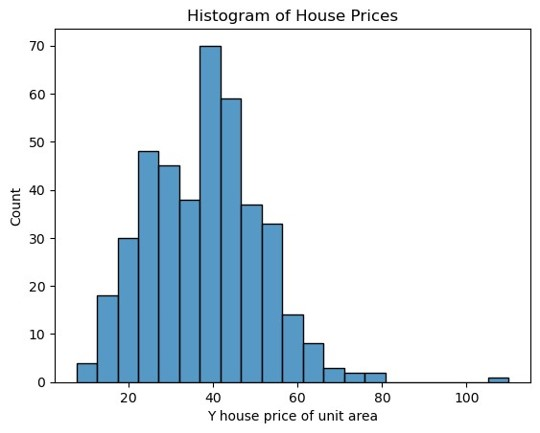
\includegraphics[width=0.8\textwidth]{histogram.png.jpg}
    \caption{Histogram of house price of unit area}
     \label{fig:histogram}
\end{figure}
\newpage
\begin{figure}[h!]
    \centering
    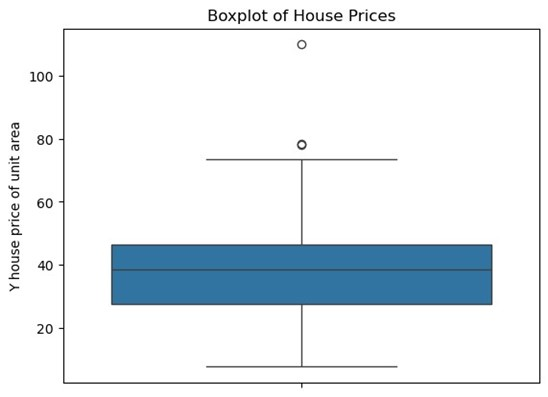
\includegraphics[width=0.8\textwidth]{boxplot.jpg}
    \caption{Histogram of house price of unit area}
     \label{fig:histogram}
\end{figure}
\vspace{-.75cm}
\begin{figure}[h!]
    \centering
    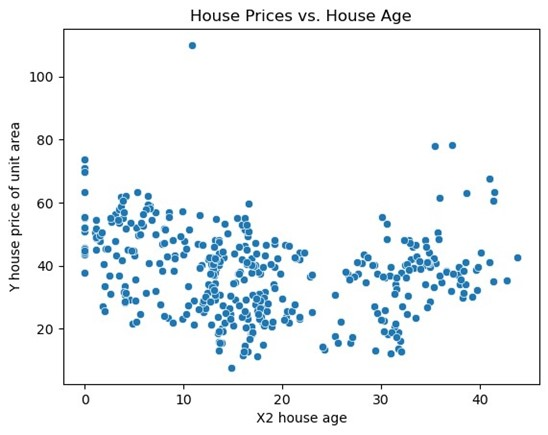
\includegraphics[width=0.8\textwidth]{scatterplot.jpg}
    \caption{Histogram of house price of unit area}
     \label{fig:histogram}
\end{figure}
\newpage
\begin{figure}[h!]
    \centering
    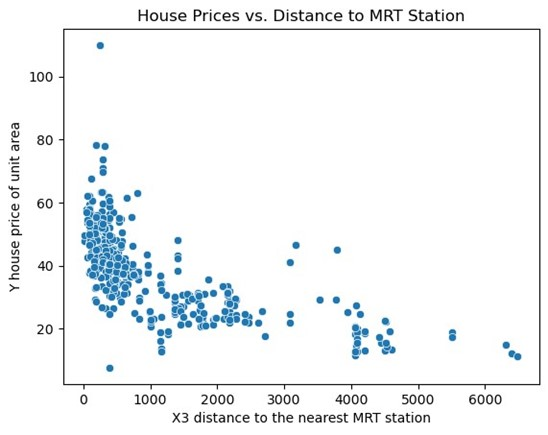
\includegraphics[width=0.8\textwidth]{scatterplot1.jpg}
    \caption{Histogram of house price of unit area}
     \label{fig:histogram}
\end{figure}
\vspace{-.75cm}
\section{Standardizing Features and Preparing Design Matrix}
\begin{code}
\begin{lstlisting}
import numpy as np
 X = np.ones((df.shape[0], 3))
 X[:, 1] = df['z_score_normalized']
 X[:, 2] = df['min_max_normalized']
 Y = df['Y house price of unit area'].values.reshape(-1, 1)
 print(X)
 print(Y)
\end{lstlisting}
\end{code}
\vspace{-.75cm}
\begin{verbatim}
  [[ 1.        -0.79458408 0.00951267] 
   [ 1.        -0.61907813 0.04380939]
   [ 1.        -0.41691656 0.08331505]
 …
 [ 1.            nan  nan]
 [ 1.            nan  nan]
 [ 1.            nan  nan]]                 
                                                            
 
 [[ 37.9]
 [ 42.2]
 [ 47.3]
 [ 54.8]
 [ 43.1]
 [ 32.1]
 [ 40.3]
 [ 46.7]
 [ 18.8]
 [ 22.1]
 [ 41.4]
 [ 58.1]
 [ 39.3]
 [ 23.8]
 [ 34.3]
 [ 50.5]
 [ 70.1]
 [ 37.4]
 [ 42.3]
 [ 47.7]
 [ 29.3]
 [ 51.6]
 [ 24.6]
 [ 47.9]
 [ 38.8]
 [ 27. ]
 [ 56.2]
 [ 33.6]
 [ 47. ]
 [ 57.1]
 [ 22.1]
 [ 25. ]
 [ 34.2]
 [ 49.3]
 [ 55.1]
 [ 27.3]
 [ 22.9]
 [ 25.3]
 [ 47.7]
 [ 46.2]
 [ 15.9]
 [ 18.2]
 [ 34.7]
 [ 34.1]
 [ 53.9]
 [ 38.3]
 [ 42. ]
 [ 61.5]
 [ 13.4]
 [ 13.2]
 [ 44.2]]
\end{verbatim}
\vspace{-.75cm}
\section{Calculating Regression Parameters Using Matrix Operations}
\begin{code}
\begin{lstlisting}
W = np.linalg.inv(X.T @ X) @ X.T @ Y
 print("Parameter Vector W (Normal Equation):", W)
\end{lstlisting}
\end{code}\begin{verbatim}
     Parameter Vector W (Normal Equation): [[nan]
 [nan]
 [nan]]
\end{verbatim}
\vspace{-.75cm}
\newpage
\section{Linear Regression with Manual Gradient Descent and TensorFlow GradientTape}
\begin{code}
\begin{lstlisting}
import numpy as np
 import tensorflow as tf
 # Example data
 X = np.random.randn(421, 2).astype(np.float32)
Y = np.random.randn(421, 1).astype(np.float32)
 # Convert to TensorFlow tensors
 X_tf = tf.convert_to_tensor(X)
 Y_tf = tf.convert_to_tensor(Y)
 # Initialize weights and bias
 W = tf.Variable(tf.random.normal((1, 2)))
 b = tf.Variable(tf.random.normal((1,)))
 # Define the loss function
 def compute_loss():
 Y_hat = tf.matmul(X_tf, W, transpose_b=True) + b
 return tf.reduce_mean(0.5 * tf.square(Y_hat- Y_tf))
 # Define the optimizer
 optimizer = tf.optimizers.SGD(learning_rate=0.01)
 # Training loop
 epochs = 1000
 for i in range(epochs):
 with tf.GradientTape() as tape:
 loss = compute_loss()
 grads = tape.gradient(loss, [W, b])
 optimizer.apply_gradients(zip(grads, [W, b]))
 print("Final Weights (TensorFlow):", W.numpy())
 print("Final Bias (TensorFlow):", b.numpy())
\end{lstlisting}
\end{code}
\begin{verbatim}
 Final Weights (TensorFlow): [[-0.01636326-0.07295796]]
 Final Bias (TensorFlow): [0.0130949]
\end{verbatim}
\section{Implementing and Using a Custom Linear Regression Class}
\begin{code}
\begin{lstlisting}
 import numpy as np
 import pandas as pd
 import tensorflow as tf
 # Create a sample DataFrame
 data = {
 'X2 house age': np.random.rand(100),
 'X3 distance to the nearest MRT station': np.random.rand(100),
 'Y house price of unit area': np.random.rand(100)
 }
 df = pd.DataFrame(data)
 # Convert DataFrame columns to TensorFlow tensors
 XT = tf.convert_to_tensor(
 df[['X2 house age', 'X3 distance to the nearest MRT station']].values,
 dtype=tf.float32
 )
 X = tf.transpose(XT) # Input matrix of shape (n, m)
 Y = tf.convert_to_tensor(
 df['Y house price of unit area'].values.reshape(1,-1),
 dtype=tf.float32
 ) # Target vector of shape (1, m)
 # Define model parameters
 m = X.shape[1] # Number of samples
 n = X.shape[0] # Number of features
 W = tf.Variable(tf.random.uniform((1, n), minval=0, maxval=1), dtype=tf.float32)
 B = tf.Variable(tf.random.uniform((1,), minval=0, maxval=1), dtype=tf.float32)
 # Training parameters
 learning_rate = 0.01
 num_iterations = 10000
 # Gradient Descent Loop
 for step in range(num_iterations):
 with tf.GradientTape() as tape:
 # Forward pass
 Y_hat = tf.matmul(W, X) + B
 error = Y_hat- Y
 loss = tf.reduce_mean(tf.square(error)) # Mean Squared Error Loss
 # Compute gradients
 grad_W, grad_B = tape.gradient(loss, [W, B])
 # Update weights and bias
 W.assign_sub(learning_rate * grad_W)
 B.assign_sub(learning_rate * grad_B)
 # Print loss and parameters at intervals
 if (step + 1) % 1000 == 0:
 print(f"Epoch {step + 1}: Loss = {loss.numpy()}, W = {W.numpy()}, B =␣
 ↪{B.numpy()}")
\end{lstlisting}
\end{code}
\begin{verbatim}
Epoch 1000: Loss = 0.08621952682733536, W = [[-0.11358874 0.10545328]], B =[0.52158034]
 Epoch 2000: Loss = 0.08483896404504776, W = [[-0.09776288 0.00779503]],
 B =[0.5688425]
 Epoch 3000: Loss = 0.08471596986055374, W = [[-0.10272954-0.01955936]],
 B =[0.5872949]
 Epoch 4000: Loss = 0.08470050990581512, W = [[-0.10686363-0.02813785]], 
 B =[0.59451085]
 Epoch 5000: Loss = 0.08469826728105545, W = [[-0.10891178-0.03107916]], 
 B =[0.597335]
 Epoch 6000: Loss = 0.08469793200492859, W = [[-0.10979746-0.03214846]], 
 B = [0.59843946]
 Epoch 7000: Loss = 0.08469788730144501, W = [[-0.11016019-0.03255066]],
 B = [0.5988717]
 Epoch 8000: Loss = 0.08469786494970322, W = [[-0.1103053-0.0327049]], B =[0.59904146]
 Epoch 9000: Loss = 0.08469786494970322, W = [[-0.11036471-0.03276638]],
 B = [0.59910977]
 Epoch 10000: Loss = 0.08469786494970322, W = [[-0.11038668-0.03278921]],
 B = [0.5991339]
\end{verbatim}




%\mychapter{1}{Assignment 5 \\ \vspace{-0.3cm} Building Machine Learning Models
with Scikit-learn}
\addcontentsline{toc}{chapter}{Assignment 5 Building Machine Learning Models
with Scikit-learn}
\usepackage{graphicx}


\section*{Problem Statement 1:Classification on the Iris Dataset}



\begin{enumerate}
    \item  Load the Iris dataset from Seaborn’s dataset module into a Pandas DataFrame.
    \item Split the dataset into training and test data.
    \item Train and evaluate the following classification models:
        \begin{enumerate}
        \item  K-Nearest Neighbors (KNN).
        \item Gaussian Naive Bayes.
        \item Decision Tree.
        \item Random Forest
        \item Support Vector Machine (SVM)
       \end{enumerate}
    \item For each model:
     \begin{enumerate}
        \item  Print the labels predicted by the model on the test data and compare them with
the actual labels.
        \item Form and display the confusion matrix using the test data.
       
    \end{enumerate}
    \section*{Problem Statement 2: K-Means Clustering on the Wine Dataset}



    \item  Load the Wine dataset from Scikit-learn’s dataset module into a Pandas DataFrame.
    \item Preprocess the data by selecting relevant features and handling any missing values
if present.
    \item Apply K-Means clustering to the dataset with the number of clusters equal to the
number of unique wine classes in the dataset.
    \item Print the cluster labels assigned to each data point by the K-Means algorithm.
    \item Compare the cluster labels with the actual wine class labels by calculating the accuracy of the clustering.
    \item Visualize the clusters using a scatter plot or pairplot with different colors representing different clusters.
        \section*{Problem Statement 3: Linear Regression on the California Housing Dataset}


    \item Load the California Housing dataset from Scikit-learn’s dataset module into a Pandas
DataFrame.
    \item Preprocess the data by selecting relevant features and handling any missing values
if present.
    \item Split the dataset into training and test data.
    \item Train a Linear Regression model on the training data.
    \item Evaluate the model by predicting housing prices on the test data and calculating
performance metrics such as Mean Squared Error (MSE) and R-squared.
   \item Print the coefficients of the model to understand the influence of each feature on the
target variable.
    
\end{enumerate}

\newpage

\vspace{-.15cm}
\section{Loading the Dataset}
\vspace{-.75cm}
\begin{code}
\begin{lstlisting}
import seaborn as sns
import pandas as pd
iris = sns.load_dataset('iris')
df = pd.DataFrame(iris)
print(df.head())
\end{lstlisting}
\end{code}
\vspace{-1cm}
\begin{verbatim} 
   sepal_length  sepal_width  petal_length  petal_width species
0           5.1          3.5           1.4          0.2  setosa
1           4.9          3.0           1.4          0.2  setosa
2           4.7          3.2           1.3          0.2  setosa
3           4.6          3.1           1.5          0.2  setosa
4           5.0          3.6           1.4          0.2  setosa

[ ]

\end{verbatim}
\vspace{-.6cm}
\section{ Split the Dataset}
\vspace{-.75cm}
\begin{code}
\begin{lstlisting}
 from sklearn.model_selection import train_test_split
train_df, test_df = train_test_split(df, test_size=0.2)
print("train data \n",train_df.head())
print("test data \n",test_df.head())
\end{lstlisting}
\end{code}
\vspace{-1cm}
\begin{verbatim}
train data 
      sepal_length  sepal_width  petal_length  petal_width     species
108           6.7          2.5           5.8          1.8   virginica
0             5.1          3.5           1.4          0.2      setosa
46            5.1          3.8           1.6          0.2      setosa
105           7.6          3.0           6.6          2.1   virginica
87            6.3          2.3           4.4          1.3  versicolor
test data 
      sepal_length  sepal_width  petal_length  petal_width     species
137           6.4          3.1           5.5          1.8   virginica
97            6.2          2.9           4.3          1.3  versicolor
13            4.3          3.0           1.1          0.1      setosa
3             4.6          3.1           1.5          0.2      setosa
93            5.0          2.3           3.3          1.0  versicolor
\end{verbatim}

\vspace{-.3cm}
\section{Load the Wine Dataset}
\vspace{-.9cm}
\begin{code}
\begin{lstlisting}
X = df.drop('species', axis=1)
y = df['species']
import pandas as pd
from sklearn.metrics import confusion_matrix, accuracy_score
import seaborn as sns
import matplotlib.pyplot as plt
from sklearn.neighbors import KNeighborsClassifier
from sklearn.naive_bayes import GaussianNB
from sklearn.tree import DecisionTreeClassifier
from sklearn.ensemble import RandomForestClassifier
from sklearn.svm import SVC

def evaluate_model(model, X_test, y_test):
  y_pred = model.predict(X_test)
  print("Predicted Labels:")
  print(y_pred)
  print("Actual Labels:")
  print(y_test)

  cm = confusion_matrix(y_test, y_pred)
  print(cm)
  accuracy = accuracy_score(y_test, y_pred)
  print(f"Accuracy: {accuracy}")

knn = KNeighborsClassifier(n_neighbors=5)
knn.fit(X_train, y_train)
print("K-Nearest Neighbors:")
evaluate_model(knn, X_test, y_test)

nb = GaussianNB()
nb.fit(X_train, y_train)
print("Gaussian Naive Bayes:")
evaluate_model(nb, X_test, y_test)

dt = DecisionTreeClassifier()
dt.fit(X_train, y_train)
print("Decision Tree:")
evaluate_model(dt, X_test, y_test)

rf = RandomForestClassifier()
rf.fit(X_train, y_train)
print("Random Forest:")
evaluate_model(rf, X_test, y_test)

 svm = SVC()
svm.fit(X_train, y_train)
print("Support Vector Machine:")
evaluate_model(svm, X_test, y_test)   
\end{lstlisting}
\end{code}
\newpage
\vspace{-1cm}
\begin{verbatim}
K-Nearest Neighbors:
Predicted Labels:
['versicolor' 'setosa' 'virginica' 'versicolor' 'versicolor' 'setosa'
 'versicolor' 'virginica' 'versicolor' 'versicolor' 'virginica' 'setosa'
 'setosa' 'setosa' 'setosa' 'versicolor' 'virginica' 'versicolor'
 'versicolor' 'virginica' 'setosa' 'virginica' 'setosa' 'virginica'
 'virginica' 'virginica' 'virginica' 'virginica' 'setosa' 'setosa']
Actual Labels:
73     versicolor
18         setosa
118     virginica
78     versicolor
76     versicolor
31         setosa
64     versicolor
141     virginica
68     versicolor
82     versicolor
110     virginica
12         setosa
36         setosa
9          setosa
19         setosa
56     versicolor
104     virginica
69     versicolor
55     versicolor
132     virginica
29         setosa
127     virginica
26         setosa
128     virginica
131     virginica
145     virginica
108     virginica
143     virginica
45         setosa
30         setosa
Name: species, dtype: object
[[10  0  0]
 [ 0  9  0]
 [ 0  0 11]]
Accuracy: 1.0
Gaussian Naive Bayes:
Predicted Labels:
['versicolor' 'setosa' 'virginica' 'versicolor' 'versicolor' 'setosa'
 'versicolor' 'virginica' 'versicolor' 'versicolor' 'virginica' 'setosa'
 'setosa' 'setosa' 'setosa' 'versicolor' 'virginica' 'versicolor'
 'versicolor' 'virginica' 'setosa' 'virginica' 'setosa' 'virginica'
 'virginica' 'virginica' 'virginica' 'virginica' 'setosa' 'setosa']
Actual Labels:
73     versicolor
18         setosa
118     virginica
78     versicolor
76     versicolor
31         setosa
64     versicolor
141     virginica
68     versicolor
82     versicolor
110     virginica
12         setosa
36         setosa
9          setosa
19         setosa
56     versicolor
104     virginica
69     versicolor
55     versicolor
132     virginica
29         setosa
127     virginica
26         setosa
128     virginica
131     virginica
145     virginica
108     virginica
143     virginica
45         setosa
30         setosa
Name: species, dtype: object
[[10  0  0]
 [ 0  9  0]
 [ 0  0 11]]
Accuracy: 1.0
Decision Tree:
Predicted Labels:
['versicolor' 'setosa' 'virginica' 'versicolor' 'versicolor' 'setosa'
 'versicolor' 'virginica' 'versicolor' 'versicolor' 'virginica' 'setosa'
 'setosa' 'setosa' 'setosa' 'versicolor' 'virginica' 'versicolor'
 'versicolor' 'virginica' 'setosa' 'virginica' 'setosa' 'virginica'
 'virginica' 'virginica' 'virginica' 'virginica' 'setosa' 'setosa']
Actual Labels:
73     versicolor
18         setosa
118     virginica
78     versicolor
76     versicolor
31         setosa
64     versicolor
141     virginica
68     versicolor
82     versicolor
110     virginica
12         setosa
36         setosa
9          setosa
19         setosa
56     versicolor
104     virginica
69     versicolor
55     versicolor
132     virginica
29         setosa
127     virginica
26         setosa
128     virginica
131     virginica
145     virginica
108     virginica
143     virginica
45         setosa
30         setosa
Name: species, dtype: object
[[10  0  0]
 [ 0  9  0]
 [ 0  0 11]]
Accuracy: 1.0
Random Forest:
Predicted Labels:
['versicolor' 'setosa' 'virginica' 'versicolor' 'versicolor' 'setosa'
 'versicolor' 'virginica' 'versicolor' 'versicolor' 'virginica' 'setosa'
 'setosa' 'setosa' 'setosa' 'versicolor' 'virginica' 'versicolor'
 'versicolor' 'virginica' 'setosa' 'virginica' 'setosa' 'virginica'
 'virginica' 'virginica' 'virginica' 'virginica' 'setosa' 'setosa']
Actual Labels:
73     versicolor
18         setosa
118     virginica
78     versicolor
76     versicolor
31         setosa
64     versicolor
141     virginica
68     versicolor
82     versicolor
110     virginica
12         setosa
36         setosa
9          setosa
19         setosa
56     versicolor
104     virginica
69     versicolor
55     versicolor
132     virginica
29         setosa
127     virginica
26         setosa
128     virginica
131     virginica
145     virginica
108     virginica
143     virginica
45         setosa
30         setosa
Name: species, dtype: object
[[10  0  0]
 [ 0  9  0]
 [ 0  0 11]]
Accuracy: 1.0
Support Vector Machine:
Predicted Labels:
['versicolor' 'setosa' 'virginica' 'versicolor' 'versicolor' 'setosa'
 'versicolor' 'virginica' 'versicolor' 'versicolor' 'virginica' 'setosa'
 'setosa' 'setosa' 'setosa' 'versicolor' 'virginica' 'versicolor'
 'versicolor' 'virginica' 'setosa' 'virginica' 'setosa' 'virginica'
 'virginica' 'virginica' 'virginica' 'virginica' 'setosa' 'setosa']
Actual Labels:
73     versicolor
18         setosa
118     virginica
78     versicolor
76     versicolor
31         setosa
64     versicolor
141     virginica
68     versicolor
82     versicolor
110     virginica
12         setosa
36         setosa
9          setosa
19         setosa
56     versicolor
104     virginica
69     versicolor
55     versicolor
132     virginica
29         setosa
127     virginica
26         setosa
128     virginica
131     virginica
145     virginica
108     virginica
143     virginica
45         setosa
30         setosa
Name: species, dtype: object
[[10  0  0]
 [ 0  9  0]
 [ 0  0 11]]
Accuracy: 1.0
\end{verbatim}

\vspace{-.75cm}
\section{ Preprocess the Data}
\vspace{-.6cm}
\begin{code}
\begin{lstlisting}
 from sklearn.datasets import load_wine
import pandas as pd

wine = load_wine()
df = pd.DataFrame(data=wine.data, columns=wine.feature_names)
df['target'] = wine.target
print(df.head())
\end{lstlisting}
\end{code}
\vspace{-.75cm}
\begin{verbatim}
    alcohol  malic_acid   ash  alcalinity_of_ash  magnesium  total_phenols  \
0    14.23        1.71  2.43               15.6      127.0           2.80   
1    13.20        1.78  2.14               11.2      100.0           2.65   
2    13.16        2.36  2.67               18.6      101.0           2.80   
3    14.37        1.95  2.50               16.8      113.0           3.85   
4    13.24        2.59  2.87               21.0      118.0           2.80   

   flavanoids  nonflavanoid_phenols  proanthocyanins  color_intensity   hue  \
0        3.06                  0.28             2.29             5.64  1.04   
1        2.76                  0.26             1.28             4.38  1.05   
2        3.24                  0.30             2.81             5.68  1.03   
3        3.49                  0.24             2.18             7.80  0.86   
4        2.69                  0.39             1.82             4.32  1.04   

   od280/od315_of_diluted_wines  proline  target  
0                          3.92   1065.0       0  
1                          3.40   1050.0       0  
2                          3.17   1185.0       0  
3                          3.45   1480.0       0  
4                          2.93    735.0       0
\end{verbatim}
\vspace{-.75cm}
\section{Apply K-Means Clustering}
\vspace{-.6cm}
\begin{code}
\begin{lstlisting}
df.isnull().sum()
df.dropna(inplace=True)
df.fillna(df.mean(), inplace=True)
from sklearn.feature_selection import SelectKBest, f_classif
selector = SelectKBest(f_classif, k=5)
X_new = selector.fit_transform(df.drop('target', axis=1), df['target'])
selected_features = df.drop('target', axis=1).columns[selector.get_support()]
df = df[selected_features]
df['target'] = wine.target
\end{lstlisting}
\end{code}
\vspace{-1cm}
\begin{verbatim}
 
                                0
alcohol	                        0
malic_acid	                     0
ash	                            0
alcalinity_of_ash	              0
magnesium	                      0
total_phenols	                  0
flavanoids	                     0
nonflavanoid_phenols        	   0
proanthocyanins             	   0
color_intensity             	   0
hue	                            0
od280/od315_of_diluted_wines	   0
proline	                        0
target	                         0
dtype: int64
\end{verbatim}
%\vspace{-.6cm}
%\newpage
\section{ Print Cluster Labels}
\begin{lstlisting}
from sklearn.cluster import KMeans

n_clusters = len(df['target'].unique())

kmeans = KMeans(n_clusters=n_clusters, random_state=42)

kmeans.fit(df.drop('target', axis=1))


labels = kmeans.labels_

df['cluster'] = labels
print(df.head())
df.to_csv('clustered_wine_data.csv', index=False)
\end{lstlisting}
\begin{verbatim}
    alcohol  flavanoids  color_intensity  od280/od315_of_diluted_wines  \
0    14.23        3.06             5.64                          3.92   
1    13.20        2.76             4.38                          3.40   
2    13.16        3.24             5.68                          3.17   
3    14.37        3.49             7.80                          3.45   
4    13.24        2.69             4.32                          2.93   

   proline  target  cluster  
0   1065.0       0        1  
1   1050.0       0        1  
2   1185.0       0        1  
3   1480.0       0        1  
4    735.0       0        0  
\end{verbatim}
\section{ Compare Cluster Labels with Actual Labels}
\begin{lstlisting}
print(df['cluster'])
\end{lstlisting}
\newpage
\begin{verbatim}
0      1
1      1
2      1
3      1
4      0
      ..
173    0
174    0
175    0
176    0
177    2
Name: cluster, Length: 178, dtype: int32                

\end{verbatim}
\section{Compare Cluster Labels with Actual Labels}
\begin{lstlisting}
print(accuracy_score(df['target'], df['cluster']))
\end{lstlisting}
\begin{verbatim}
 0.1853932584269663                

\end{verbatim}
\section{Visualize the Clusters}
\begin{lstlisting}
import seaborn as sns
import matplotlib.pyplot as plt

sns.pairplot(df, hue='cluster', palette='viridis')
plt.show()
\end{lstlisting}

\newpage

\begin{figure}[h!]
    \centering
    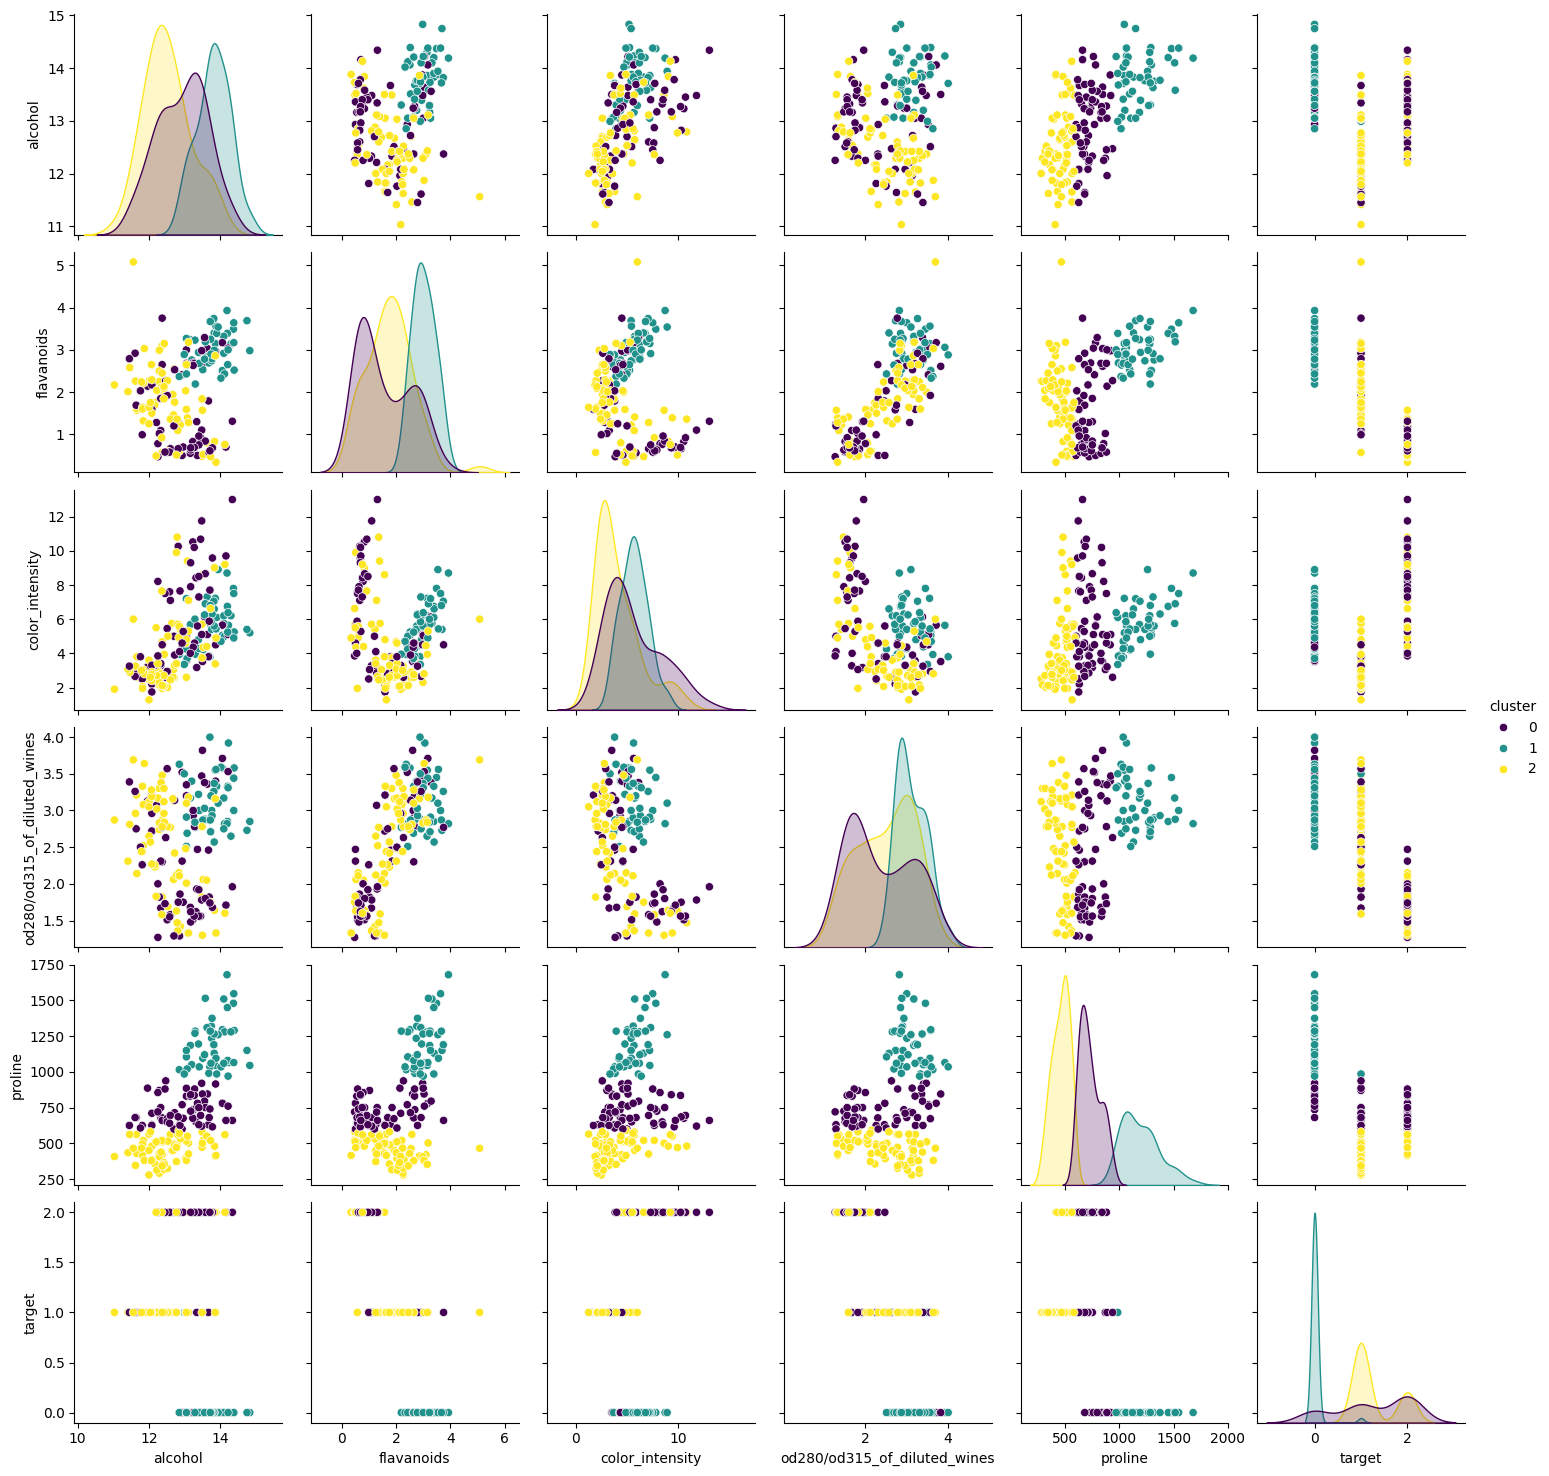
\includegraphics[width=0.8\textwidth]{download.png}
    \caption{}
     \label{}
\end{figure}            


\section*{Problem Statement 3: Linear Regression on the California Housing Dataset}
\section{ Load the California Housing Dataset}
\begin{lstlisting}
 from sklearn.datasets import fetch_california_housing 
import pandas as pd
housing = fetch_california_housing() 
df = pd.DataFrame(data=housing.data, columns=housing.feature_names) 
df['target'] = housing.target 
print(df.head()) 
\end{lstlisting}
\begin{verbatim}
    MedInc  HouseAge  AveRooms  AveBedrms  Population  AveOccup  Latitude  \ 
0  8.3252      41.0  6.984127   1.023810       322.0  2.555556     37.88    
1  8.3014      21.0  6.238137   0.971880      2401.0  2.109842     37.86    
2  7.2574      52.0  8.288136   1.073446       496.0  2.802260     37.85    
3  5.6431      52.0  5.817352   1.073059       558.0  2.547945     37.85    
4  3.8462      52.0  6.281853   1.081081       565.0  2.181467     37.85    
   Longitude  target   
0    -122.23   4.526   
1    -122.22   3.585   
2    -122.24   3.521   
3    -122.25   3.413   
4    -122.25   3.422   
\end{verbatim}
\section{Preprocess the Data}
\begin{lstlisting}
 df.isnull().sum() 
df.fillna(df.mean(), inplace=True) 
from sklearn.feature_selection import SelectKBest, f_regression 
selector = SelectKBest(f_regression, k=5)  
X_new = selector.fit_transform(df.drop('target', axis=1), df['target']) 
selected_features = df.drop('target', axis=1).columns[selector.get_support()] 
\end{lstlisting}
\section{Split the Dataset}
\begin{lstlisting}
    X_train, X_test, y_train, y_test = train_test_split(X_california, y_california, test_size=0.3, random_state=42)
\end{lstlisting}

\section{ Train a Linear Regression Model}
\begin{lstlisting}
 from sklearn.model_selection import train_test_split 
X = df.drop('target', axis=1) 
y = df['target'] 
X_train, X_test, y_train, y_test = train_test_split(X, y, test_size=0.2, random_s
 from sklearn.linear_model import LinearRegression 
model = LinearRegression() 
model.fit(X_train, y_train) 
\end{lstlisting}
\begin{verbatim}
▾ LinearRegression
 LinearRegression()        
\end{verbatim}
\section{Evaluate the Model}
\begin{lstlisting}
 from sklearn.metrics import mean_squared_error, r2_score 
y_pred = model.predict(X_test) 
mse = mean_squared_error(y_test, y_pred) 
r2 = r2_score(y_test, y_pred) 
print(f'Mean Squared Error: {mse}') 
print(f'R-squared: {r2}')
\end{lstlisting}
\begin{verbatim}
Mean Squared Error: 0.6382565441555921 
R-squared: 0.5129333248216971         
\end{verbatim}
\section{ Print the Coefficients}
\begin{lstlisting}
 print(f'Coefficients: {model.coef_}')
 print(df[['X3 distancetothenearestMRTstation','decimal_scaled']].head())
\end{lstlisting}
\begin{verbatim}
Coefficients: [ 0.53520156  0.01618449 -0.20927062  1.050567   -0.03105515] 
\end{verbatim}

  





%\mychapter{1}{Assignment 6 \\ \vspace{-0.3cm} Implementing an FCNN from
Scratch using TensorFlow}
\addcontentsline{toc}{chapter}{Assignment 6 Implementing an FCNN from Scratch using TensorFlow}



\section*{Problem Statement: } \\
\item Implement the following computations using TensorFlow:
\begin{document}
%\thispagestyle{bordered}


\begin{enumerate}
    \item  Load the the MNIST dataset from tensorflow as x train, y train, x test and y test.
The Modified National Institute of Standards and Technology (MNIST) dataset
contains grayscale images of handwritten digits. The training set consists of 60,000
images and the test set contains 10,000 images. The label of each image is a digit
between 0 and 9. Each image has a size of 28 × 28, consisting of 784 pixel values,
where each pixel value ∈ [0, 255] with 0 corresponds to black, 255 to white, and
values in between representing various shades of gray.
    \item Compute X as the transpose of U.

    \item Normalize the pixel values of X to [0, 1] by dividing by 255.

    \item Form a matrix Y of size m corresponding to the labels ∈ [0, 9] of images by transposing y train.

    \item Form a matrix V by reshaping the images in x test to be 1D arrays of 784 (28 × 28)
pixel values (Flatten the images).

    \item Compute Xtest as the transpose of V .

    \item Normalize the pixel values of Xtest to [0, 1] by dividing by 255.

    \item Form a matrix Y test of size m corresponding to the labels ∈ [0, 9] of images by
transposing y test.

    \item Select an image from X and display it. Also, display the corresponding label from
Y.

    \item Form a matrix Y of size m corresponding to the labels ∈ [0, 9] of images by transposing y train.

    \item Set the hyper parameters: p = 10, the no. of neurons in hidden layer, q = 10,
the no. of neurons in output layer (corresponding 10 labels in one-hot encoding
format), learning rate α = 0.01 and the number of training epochs (iterations over
the dataset) as 1000.

    \item Create a matrix W1 of shape (p, n) and initialize it as W1 = N (0, 1) ×
q
1
n
, where
N (0, 1) represents a matrix of random values drawn from a normal distribution with
mean 0 and standard deviation 1.

    \item Initialize the vector B1 of shape (p, 1) to zeros.

    \item Initialize the matrix $W_2$ of shape $(q, p)$ as $W_2 = \mathcal{N}(0, 1) \times \frac{q_1}{p}$.

    \item Initialize the vector B2 of shape (q, 1) to zeros.

    \item Perform the following forward propagation and backpropagation computations iteratively (No. of epochs=1000):
        \begin{enumerate}
        \item  Z1 = W1 · X + B1 (Matrix Multiplication)
        \item A1 = ReLU(Z1) where ReLU(x) is a function that returns 0 for negative values
and the input value itself otherwise.

        \item Z2 = W2 · A1 + B2
        \item $A_2 = \text{softmax}(Z_2)$, where $\text{softmax}(x) = \frac{e^{x_i}}{\sum_j e^{x_j}}$.

        \item Get the predicted labels from the output of A2 (index of the maximum value).

        \item Find the accuracy of the predictions by comparing them to the true labels Y
and print the progress in every 100 epochs.

        \item Compute the cross-entropy loss using TensorFlow’s tf.nn.softmax cross entropy with logits
function.

        \item  dZ2 = A2 − one hot Y where one hot Y is the one-hot encoded form of Y .

        \item $dA_2 = W_2^T \cdot dZ_2$


        \item $dW_2 = \frac{1}{m} \cdot dZ_2 \cdot A_1^T$


        \item $dB_2 = \frac{1}{m} \sum dZ_2 \,\, (\text{sum along the columns})$
 

        \item dZ1 = dA2◦ReLU deriv(Z1) where ReLU deriv(x) returns 1 for positive values
and 0 otherwise, and ◦ indicates element-wise multiplication.

        \item $dA_1 = W_1^T \cdot dZ_1$

        \item $dB_1 = \frac{1}{m} \sum dZ_1 \quad \text{(sum along the columns)}$

        \item $dW_1 = \frac{1}{m} \cdot dZ_1 \cdot X^T$

        \item (p) Update and print $W_1$, $B_1$, $W_2$, and $B_2$ for $\alpha = 0.01$:
            \begin{enumerate}[i.]
                \item $W_1 = W_1 - \alpha \cdot dW_1$
                \item $B_1 = B_1 - \alpha \cdot dB_1$
                \item $W_2 = W_2 - \alpha \cdot dW_2$
                \item $B_2 = B_2 - \alpha \cdot dB_2$
            \end{enumerate}
       \end{enumerate}

       \item . Use tensorflow GradientTape() to automatically calculate the gradients from steps
(h) to (o) and redo the training steps.

        \item Select one test image from Xtest, display it, reshape it to n × 1, perform forward
propagation computations and predict the label. Check whether the prediction is
correct.

    \item Use the entire Xtest and perform the forward propagation computations and predict
the accuracy of the model.

\end{enumerate}

\newpage

\vspace{-.15cm}
\section{Load and Preprocess Data}
\vspace{-.75cm}
\begin{code}
\begin{lstlisting}
import numpy as np
from matplotlib import pyplot as plt
import tensorflow as tf
(x_train, y_train), (x_test, y_test) = tf.keras.datasets.mnist.load_data()
U = tf.reshape(x_train, (x_train.shape[0], 784))
X = tf.transpose(U)
X = tf.cast(X, tf.float32) / 255.0
Y = tf.transpose(tf.convert_to_tensor(y_train))
n, m = X.shape
V = tf.reshape(x_test, (x_test.shape[0], 784))
Xtest = tf.transpose(V)
Xtest = tf.cast(Xtest, tf.float32) / 255.0
Ytest = tf.transpose(tf.convert_to_tensor(y_test))
\end{lstlisting}
\end{code}
\vspace{-1cm}
\begin{verbatim} 
Downloading data from https://storage.googleapis.com/tensorflow/tf-keras-datasets/mnist.npz
11490434/11490434 0s 0us/step

\end{verbatim}
\vspace{-.6cm}
\section{ Display an Image}
\vspace{-.75cm}
\begin{code}
\begin{lstlisting}
ind = 0
image = X[:, ind]
image = tf.reshape(image, (28, 28)) * 255
image_np = image.numpy()
plt.imshow(image_np, cmap='gray', interpolation='nearest')
print(f"Label: {Y[ind].numpy()}")
plt.show()
\end{lstlisting}
\end{code}
\vspace{-1cm}
    \begin{figure}[h!]
        \centering
        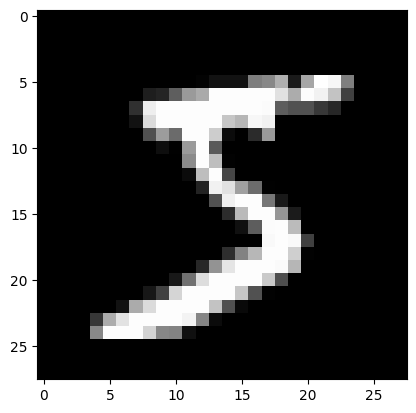
\includegraphics[width=8cm, height=8cm]{ass6pic.png}
        \caption{Image Visualization}
        \label{fig:image_visualization}
    \end{figure}         

    \vspace{-.3cm}

\newpage
\vspace{-.3cm}
\section{Neural Network Parameters}
\vspace{-.9cm}
\begin{code}
\begin{lstlisting}
p = 10
c = 10
alpha = 0.01
epoch = 1000
W1 = tf.Variable(tf.random.normal((p, n), stddev=tf.math.sqrt(1. / n)))
b1 = tf.Variable(tf.zeros((p, 1)))
W2 = tf.Variable(tf.random.normal((c, p), stddev=tf.math.sqrt(1. / p)))
b2 = tf.Variable(tf.zeros((c, 1)))  
\end{lstlisting}
\end{code}

\vspace{-1cm}
\begin{verbatim}
\end{verbatim}

\vspace{-.75cm}
\section{ Activation Functions and Encoding}
\vspace{-.6cm}
\begin{code}
\begin{lstlisting}
def ReLU(Z):
return tf.maximum(Z, 0)
def ReLU_deriv(Z):
return tf.cast(Z > 0, dtype=tf.float32)
def softmax(Z):
exp_Z = tf.exp(Z - tf.reduce_max(Z))
return exp_Z / tf.reduce_sum(exp_Z, axis=0, keepdims=True)
def one_hot(Y):
return tf.one_hot(Y, depth=tf.reduce_max(Y) + 1)
\end{lstlisting}
\end{code}
\vspace{-.75cm}
\begin{verbatim}

\end{verbatim}
\vspace{-.75cm}
\section{Training Loop}
\vspace{-.6cm}
\begin{code}
\begin{lstlisting}
for i in range(epoch):
Z1 = tf.matmul(W1, X) + b1
A1 = ReLU(Z1)
Z2 = tf.matmul(W2, A1) + b2
A2 = softmax(Z2)
one_hot_Y = one_hot(tf.cast(Y, dtype=tf.int32))
one_hot_Y = tf.transpose(one_hot_Y)
if i % 100 == 0:
yhat = tf.argmax(A2, axis=0)
accuracy=tf.reduce_mean(tf.cast(yhat==tf.cast(Y,dtype=tf.int64),dtype=tf.float32)).numpy() * 100
print(f"Epoch: {i}, Accuracy: {accuracy:.2f}%")
\end{lstlisting}
\end{code}
\begin{code}
\begin{lstlisting}
dZ2 = A2 - one_hot_Y
dW2 = 1 / m * tf.matmul(dZ2, tf.transpose(A1))
db2 = 1 / m * tf.reduce_sum(dZ2, axis=1, keepdims=True)
dA2 = tf.matmul(tf.transpose(W2), dZ2)
dZ1 = dA2 * ReLU_deriv(Z1)
dW1 = 1 / m * tf.matmul(dZ1, tf.transpose(X))
db1 = 1 / m * tf.reduce_sum(dZ1, axis=1, keepdims=True)
W2.assign(W2 - alpha * dW2)
b2.assign(b2 - alpha * db2)
W1.assign(W1 - alpha * dW1)
b1.assign(b1 - alpha * db1)
\end{lstlisting}
\end{code}
\vspace{-1cm}
\begin{verbatim}







Epoch: 0, Accuracy: 7.20%
Epoch: 100, Accuracy: 31.82%
Epoch: 200, Accuracy: 47.35%
Epoch: 300, Accuracy: 66.75%
Epoch: 400, Accuracy: 74.39%
Epoch: 500, Accuracy: 78.53%
Epoch: 600, Accuracy: 80.75%
Epoch: 700, Accuracy: 82.20%
Epoch: 800, Accuracy: 83.30%
Epoch: 900, Accuracy: 84.22%
\end{verbatim}
%\vspace{-.6cm}
%\newpage
\section{Make Predictions}
\begin{lstlisting}
def show_prediction(index, W1, b1, W2, b2):
testimage = Xtest[:, index]
testimage = tf.reshape(testimage, (784, 1))
Z1 = tf.matmul(W1, testimage) + b1
A1 = ReLU(Z1)
Z2 = tf.matmul(W2, A1) + b2
A2 = softmax(Z2)
yhat = tf.argmax(A2, axis=0).numpy()
label = Ytest[index].numpy()
testimage = tf.reshape(testimage, (28, 28)) * 255
plt.gray()
plt.imshow(testimage, interpolation='nearest')
plt.show()
print("Prediction:", yhat)
print("Actual Label:", label)
index=39
show_prediction(index, W1, b1, W2, b2)
\end{lstlisting}


\vspace{-1cm}
    \begin{figure}[h!]
        \centering
        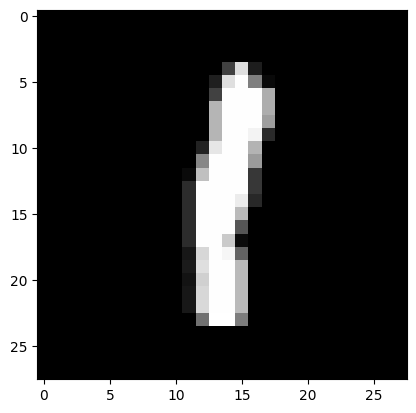
\includegraphics[width=8cm, height=8cm]{ass6pic2.png}
        \caption{Image Visualization}
        \label{fig:image_visualization}
    \end{figure}         

    \vspace{-.3cm}  

\section{Evaluate Model}
\begin{lstlisting}
def test(Xtest, Ytest, W1, b1, W2, b2):
Z1 = tf.matmul(W1, Xtest) + b1
A1 = ReLU(Z1)
Z2 = tf.matmul(W2, A1) + b2
A2 = softmax(Z2)
yhat = tf.argmax(A2, axis=0).numpy()
accu = tf.reduce_mean(tf.cast(tf.equal(yhat, Ytest), dtype=tf.float32)).numpy() * 100
print("Predictions:", yhat)
print("Actual Labels:", Ytest.numpy())
print("Accuracy:", accu, "%")
test(Xtest,Ytest,W1,b1,W2,b2)
\end{lstlisting}
\begin{verbatim}
 Predictions: [7 2 1 ... 4 8 6]
Actual Labels: [7 2 1 ... 4 5 6]
Accuracy: 85.6000006198883 %
\end{verbatim}
\newpage
\section{Error, Precision, Recall,f1 score}
\begin{lstlisting}
from sklearn.metrics import confusion_matrix, precision_score, recall_score, f1_score
def test_and_evaluate(Xtest, Ytest, W1, b1, W2, b2):
Z1 = tf.matmul(W1, Xtest) + b1
A1 = ReLU(Z1)
Z2 = tf.matmul(W2, A1) + b2
A2 = softmax(Z2)
yhat = tf.argmax(A2, axis=0).numpy()
y_true = Ytest.numpy()
cm = confusion_matrix(y_true, yhat)
error_rate = 1 - np.trace(cm) / np.sum(cm)
precision = precision_score(y_true, yhat, average='weighted')
recall = recall_score(y_true, yhat, average='weighted')
f1 = f1_score(y_true, yhat, average='weighted')
print("Confusion Matrix:\n", cm)
print("Error Rate:", error_rate)
print("Precision:", precision)
print("Recall:", recall)
print("F1 Score:", f1)
test_and_evaluate(Xtest, Ytest, W1, b1, W2, b2)
\end{lstlisting}
\begin{verbatim}              
Confusion Matrix:
[[ 935 0 2 6 1 8 17 2 9 0]
[ 0 1103 2 5 1 0 4 1 19 0]
[ 18 23 849 50 20 1 29 19 19 4]
[ 10 6 35 839 2 45 7 10 38 18]
[ 1 9 6 0 831 2 13 0 12 108]
[ 24 15 7 95 30 634 24 15 32 16]
[ 24 8 7 0 13 20 877 0 9 0]
[ 8 41 28 3 9 1 1 881 12 44]
[ 5 29 8 38 23 25 14 19 795 18]
[ 10 11 9 7 94 20 1 26 15 816]]
Error Rate: 0.14400000000000002
Precision: 0.8560334612260678
Recall: 0.856
F1 Score: 0.8549597853086216
\end{verbatim}
%\input{program2_2.tex}
%\input{program2_3.tex}
%\input{program2_4.tex}
%\input{program3_1.tex}
%\input{program4_1.tex}
%\input{program4_2.tex}
%\input{program4_3.tex}

\end{document}

